%--------------------------------------------------------------------------
%--------------------------------------------------------------------------
%--------------------------------------------------------------------------
\chapter{Tris rapides}
%--------------------------------------------------------------------------
%--------------------------------------------------------------------------
%--------------------------------------------------------------------------
%--------------------------------------------------------------------------
\section{Retour sur les tris classiques}
%--------------------------------------------------------------------------
%--------------------------------------------------------------------------
%--------------------------------------------------------------------------
La dernière étape du tri par insertion d'une liste de taille $n$ consiste à 
%--------------------------------------------------------------------------
\begin{enumerate}
\item trier les $n-1$ premier éléments,
\item insérer le dernier élément.
\end{enumerate}
%--------------------------------------------------------------------------
On peut voir le tri par sélection d'une liste de taille $n$ sous la forme
%--------------------------------------------------------------------------
\begin{enumerate}
\item on choisit le plus petit élément et on le place en tête
\item on trie les $n-1$ derniers éléments.
\end{enumerate}
%--------------------------------------------------------------------------
Ces écritures sont, de manière essentielle, récursives. 

On a laissé dans le flou la signification de "{\it trier les $n-1$ premiers éléments}" et "{\it on trie les $n-1$ derniers éléments}", les détails sont demandés dans les exercices du chapitre précédent.

On peut rassembler les deux algorithmes sous la forme 
%--------------------------------------------------------------------------
\begin{enumerate}
\item On sépare un élément du reste :
\begin{itemize}
\item le dernier élément dans le cas du tri par insertion,
\item le plus petit élément dans le cas du tri par sélection.
\end{itemize} 
\item On trie les éléments restants de manière récursive.
\item On ajoute l'élément séparé : 
\begin{itemize}
\item on l'insère dans le cas du tri par insertion,
\item c'est automatique dans le cas du tri par sélection.
\end{itemize}
\end{enumerate}
%--------------------------------------------------------------------------
On va généraliser ce schéma en n'imposant plus de couper la liste de taille $n$ en un élément et une liste de taille $n - 1$ mais en séparant en deux parties de tailles quelconques.
%--------------------------------------------------------------------------
\begin{enumerate}
\item On sépare la liste en deux sous-listes \type{l1} et \type{l2}.
\item On trie \type{l1} et \type{l2} de manière récursive
\item On assemble \type{l1} et \type{l2} pour obtenir une liste triée.
\end{enumerate}
%--------------------------------------------------------------------------
\begin{center}
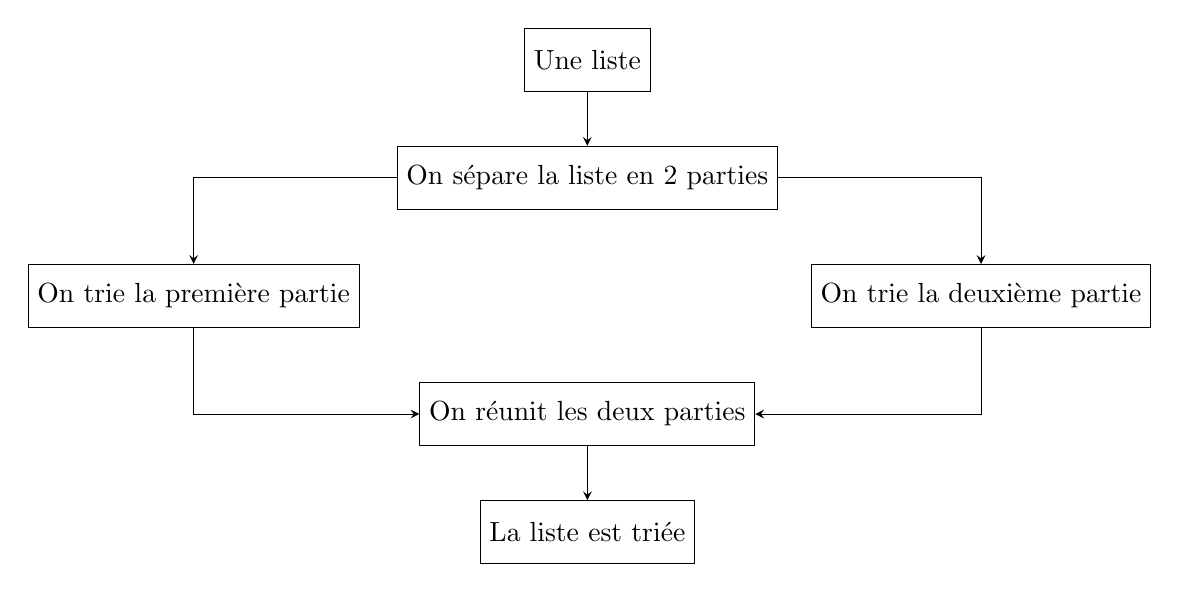
\begin{tikzpicture}[>=stealth]
\node[draw] (in) at (0,1.5) {Une liste};
\node[draw] (sep) at (0,0) {On sépare la liste en 2 parties};
\node[draw] (tri1) at (-5,-1.5) {On trie la première partie};
\node[draw] (tri2) at  (5,-1.5) {On trie la deuxième partie};
\node[draw] (union) at  (0,-3) {On réunit les deux parties};
\node[draw] (out) at (0,-4.5) {La liste est triée};
\draw[->] (in) -- (sep);
\draw[->] (sep) -| (tri1);
\draw[->] (sep) -| (tri2);
\draw[->] (tri1) |- (union);
\draw[->] (tri2) |- (union);
\draw[->] (union) -- (out);
\end{tikzpicture}
\end{center}
%--------------------------------------------------------------------------
Dans le cas du tri par insertion la séparation est facile, on isole un terme mais l'assemblage est difficile car on doit insérer ce terme à sa place.

Par contre, dans le cas du tri par sélection, la séparation est difficile, on doit chercher la plus petit élément mais l'assemblage est facile car les élément sont à leur place.


Il serait idéal de trouver un tri pour lequel séparation et assemblage sont simples mais cela semble impossible. Nous allons proposer deux tris : pour l'un la séparation est immédiate mais l'assemblage est difficile, c'est le tri-fusion,  pour l'autre la séparation sera la partie coûteuse, c'est le tri rapide.
%--------------------------------------------------------------------------
\begin{center}
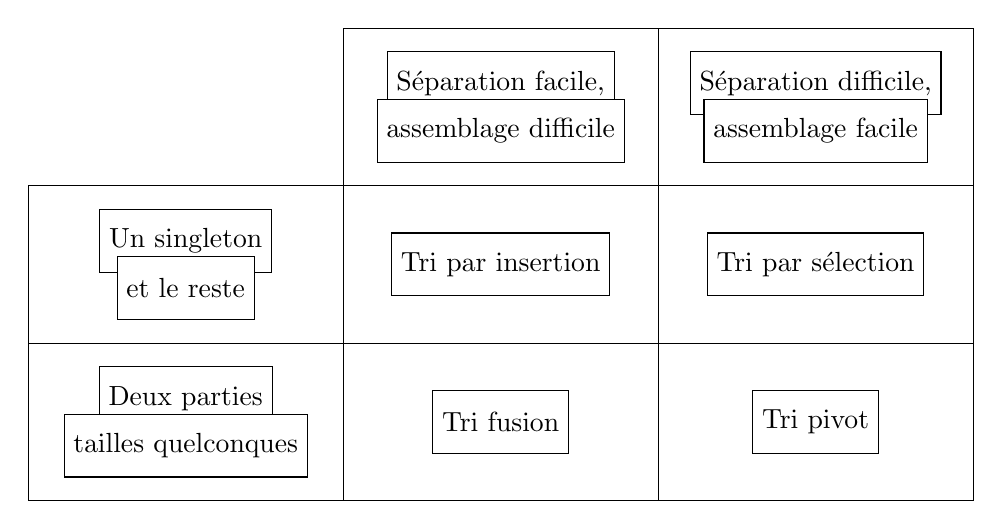
\begin{tikzpicture}[>=stealth]
\draw(0,2) rectangle (4,-4);
\draw(4,2) rectangle (8,-4);
\draw (-4,0)  rectangle (8,-2);
\draw (-4,-2) rectangle (8,-4);
\node at (2,1.3) {Séparation facile,};
\node at (2,0.7) {assemblage difficile};
\node at (6,1.3) {Séparation difficile,};
\node at (6,0.7) {assemblage facile};
\node at (-2,-0.7) {Un singleton};
\node at (-2,-1.3) {et le reste};
\node at (-2,-2.7) {Deux parties};
\node at (-2,-3.3) {tailles quelconques};
\node at (2,-1) {Tri par insertion};
\node at (6,-1) {Tri par sélection};
\node at (2,-3) {Tri fusion};
\node at (6,-3) {Tri pivot};
\end{tikzpicture}
\end{center}


\medskip

On supposera que les éléments des listes à trier sont comparés à l'aide d'une fonction, nommée \type{plusGrand}, qui renvoie \type{True} si le premier argument est supérieur (ou égal) au second.

Dans le cas d'éléments simples, la fonction \type{plusGrand} est simple aussi
%----------------------------------------------------------------
\begin{lstlisting}
def plusGrand(x1, x2):
    """Entree : deux nombres
       Sortie : True ou False selon que x1 > x2 ou non"""
    return x1 > x2
\end{lstlisting}
%--------------------------------------------------------------------------
\newpage
%--------------------------------------------------------------------------
%--------------------------------------------------------------------------
\section{Tri-fusion}
%--------------------------------------------------------------------------
%--------------------------------------------------------------------------
\subsection{Principe}
%--------------------------------------------------------------------------
%--------------------------------------------------------------------------
Le tri-fusion est une application du principe {\bf diviser pour régner} : on sépare les données en deux parts presque égales, on traite chaque partie, on rassemble.

%--------------------------------------------------------------------------
\begin{center}
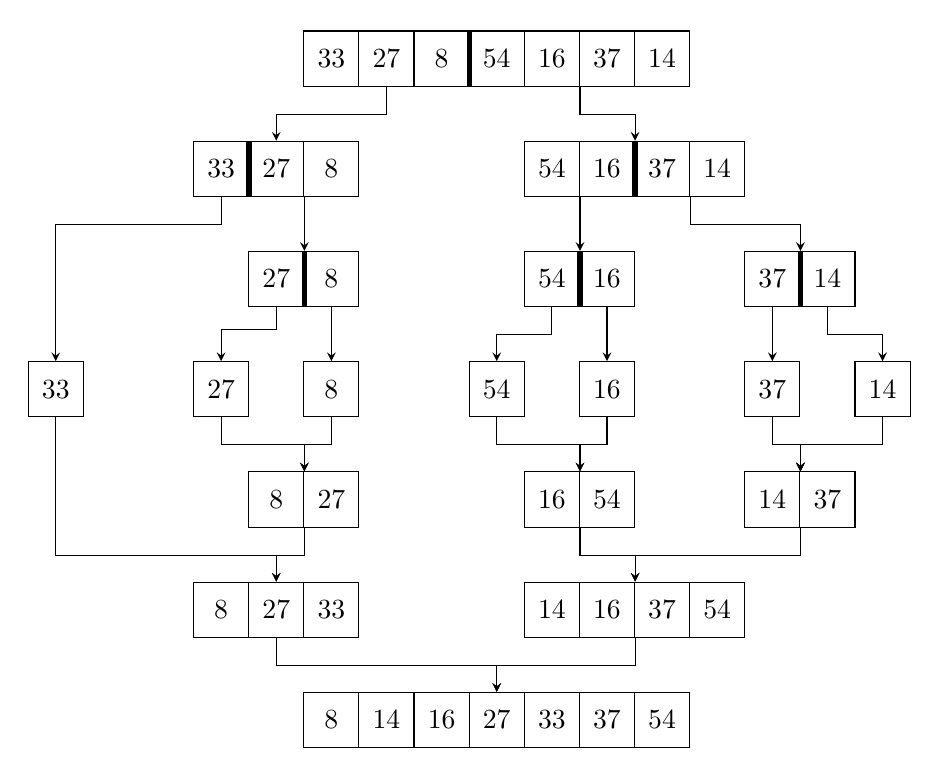
\begin{tikzpicture}[>=stealth, scale=0.7]
\tikzstyle{every node}=[draw,minimum size =7mm,fill=white]
\node[rectangle](l00) at (0,6) {33};
\node[rectangle](l01) at (1,6) {27};
\node[rectangle](l02) at (2,6) {8};
\node[rectangle](l03) at (3,6) {54};
\node[rectangle](l04) at (4,6) {16};
\node[rectangle](l05) at (5,6) {37};
\node[rectangle](l06) at (6,6) {14};
\draw[line width=2pt] (l02.north east) -- (l02.south east);
%
\node[rectangle](l10) at (-2,4) {33};
\node[rectangle](l11) at (-1,4) {27};
\node[rectangle](l12) at (0,4) {8};
\node[rectangle](l13) at (4,4) {54};
\node[rectangle](l14) at (5,4) {16};
\node[rectangle](l15) at (6,4) {37};
\node[rectangle](l16) at (7,4) {14};
\draw[line width=2pt] (l10.north east) -- (l10.south east);
\draw[line width=2pt] (l14.north east) -- (l14.south east);
%
%\node[rectangle](l20) at (-5,2) {33};
\node[rectangle](l21) at (-1,2) {27};
\node[rectangle](l22) at (0,2) {8};
\node[rectangle](l23) at (4,2) {54};
\node[rectangle](l24) at (5,2) {16};
\node[rectangle](l25) at (8,2) {37};
\node[rectangle](l26) at (9,2) {14};
\draw[line width=2pt] (l21.north east) -- (l21.south east);
\draw[line width=2pt] (l23.north east) -- (l23.south east);
\draw[line width=2pt] (l25.north east) -- (l25.south east);
%
\node[rectangle](l30) at (-5,0) {33};
\node[rectangle](l31) at (-2,0) {27};
\node[rectangle](l32) at (0,0) {8};
\node[rectangle](l33) at (3,0) {54};
\node[rectangle](l34) at (5,0) {16};
\node[rectangle](l35) at (8,0) {37};
\node[rectangle](l36) at (10,0) {14};
%
\draw[->] (l01.south) -- +(0,-0.5) -|  (l11.north);
\draw[->] (l04.south east) -- +(0,-0.5) -|  (l14.north east);
\draw[->] (l10.south) -- +(0,-0.5) -|  (l30.north);
\draw[->] (l11.south east) -- +(0,-0.5) -|  (l21.north east);
\draw[->] (l13.south east) -- +(0,-0.5) -|  (l23.north east);
\draw[->] (l15.south east) -- +(0,-0.5) -|  (l25.north east);
%\draw[->] (l20.south) -- (l30.north);
\draw[->] (l21.south) -- +(0,-0.4) -|  (l31.north);
\draw[->] (l22.south) -- (l32.north);
\draw[->] (l23.south) -- +(0,-0.5) -|  (l33.north);
\draw[->] (l24.south) -- +(0,-0.5) -|  (l34.north);
\draw[->] (l25.south) -- +(0,-0.5) -|  (l35.north);
\draw[->] (l26.south) -- +(0,-0.5) -|  (l36.north);
%
\node[rectangle](l60) at (0,-6) {8};
\node[rectangle](l61) at (1,-6) {14};
\node[rectangle](l62) at (2,-6) {16};
\node[rectangle](l63) at (3,-6) {27};
\node[rectangle](l64) at (4,-6) {33};
\node[rectangle](l65) at (5,-6) {37};
\node[rectangle](l66) at (6,-6) {54};
%
\node[rectangle](l40) at (-2,-4) {8};
\node[rectangle](l41) at (-1,-4) {27};
\node[rectangle](l42) at  (0,-4) {33};
\node[rectangle](l43) at  (4,-4) {14};
\node[rectangle](l44) at  (5,-4) {16};
\node[rectangle](l45) at  (6,-4) {37};
\node[rectangle](l46) at  (7,-4) {54};
%
\node[rectangle](l51) at (-1,-2) {8};
\node[rectangle](l52) at  (0,-2) {27};
\node[rectangle](l53) at  (4,-2) {16};
\node[rectangle](l54) at  (5,-2) {54};
\node[rectangle](l55) at  (8,-2) {14};
\node[rectangle](l56) at  (9,-2) {37};
%
%\draw[->] (l30.south) -- (l20.north);
\draw[->] (l31.south) -- +(0,-0.5) -|  (l51.north east);
\draw[->] (l32.south) -- +(0,-0.5) -|  (l51.north east);
\draw[->] (l33.south) -- +(0,-0.5) -|  (l53.north east);
\draw[->] (l34.south) -- +(0,-0.5) -|  (l53.north east);
\draw[->] (l35.south) -- +(0,-0.5) -|  (l55.north east);
\draw[->] (l36.south) -- +(0,-0.5) -|  (l55.north east);
\draw[->] (l36.south) -- +(0,-0.5) -|  (l55.north east);
\draw[->] (l30.south) -- +(0,-2.5) -|  (l41.north);
\draw[->] (l51.south east) -- +(0,-0.5) -|  (l41.north);
\draw[->] (l53.south east) -- +(0,-0.5) -|  (l44.north east);
\draw[->] (l55.south east) -- +(0,-0.5) -|  (l44.north east);
\draw[->] (l41.south) -- +(0,-0.5) -|  (l63.north);
\draw[->] (l44.south east) -- +(0,-0.5) -|  (l63.north);
\end{tikzpicture}
\end{center}
%--------------------------------------------------------------------------

On montre les détails de la dernière étape à la page suivante.
%--------------------------------------------------------------------------
%--------------------------------------------------------------------------
\subsection{Écriture en python}
%--------------------------------------------------------------------------
%--------------------------------------------------------------------------
Lors de la séparation de la liste en deux, la taille des listes diminue sauf dans le cas d'une liste de longueur  0 ou 1. C'est un cas terminal,dans ce cas on renvoie une copie de la liste.

On voit que les éléments sont placés sans qu'il semble possible de le faire avec des échanges simples ; on les place dans une nouvelle liste, ce qui impose de définir des listes supplémentaires.
%----------------------------------------------------------------
\begin{lstlisting}[caption = Tri fusion externe]
def triFusion(liste):
    """Entree : une liste
       Sortie : une liste triée avec les mêmes éléments"""
    n = len(liste)
    if n <= 1:
        return deepcopy(liste)
    else:
        l1 = triFusion(liste[0:n//2])
        l2 = triFusion(liste[n//2:n])
        return fusion(l1,l2)
\end{lstlisting}
%--------------------------------------------------------------------------

Il reste à écrire la fusion de deux liste ordonnées.
L'idée, illustrée à la page suivante,  est de placer, dans l'ordre, les éléments des deux listes en choisissant le plus petit des éléments non encore placés.

\newpage

Dans l'exemple les 5 premiers éléments sont ajoutés en comparant effectivement les premiers éléments non encore utilisés dans chaque liste. Par contre les deux derniers éléments sont placés sans comparaison car la première liste a complètement été placée.
%--------------------------------------------------------------------------
\begin{center}
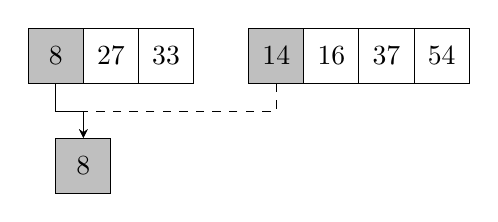
\begin{tikzpicture}[>=stealth, scale=0.7]
\tikzstyle{every node}=[draw,minimum size =7mm,fill=white]
\node[rectangle,fill=lightgray](l00) at (0,4) {8};
\node[rectangle](l01) at (1,4) {27};
\node[rectangle](l02) at (2,4) {33};
\node[rectangle,fill=lightgray](l03) at (4,4) {14};
\node[rectangle](l04) at (5,4) {16};
\node[rectangle](l05) at (6,4) {37};
\node[rectangle](l06) at (7,4) {54};
\node[rectangle,fill=lightgray](t00) at (0.5,2) {8};
\draw[->] (l00.south) -- +(0,-0.5) -| (t00.north);
\draw[->,dashed] (l03.south) -- +(0,-0.5) -|  (t00.north);
\end{tikzpicture}
\end{center}
%--------------------------------------------------------------------------
\vskip 4mm
%--------------------------------------------------------------------------
\begin{center}
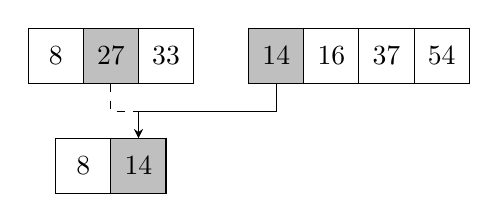
\begin{tikzpicture}[>=stealth, scale=0.7]
\tikzstyle{every node}=[draw,minimum size =7mm,fill=white]
\node[rectangle](l10) at (0,0) {8};
\node[rectangle,fill=lightgray](l11) at (1,0) {27};
\node[rectangle](l12) at (2,0) {33};
\node[rectangle,fill=lightgray](l13) at (4,0) {14};
\node[rectangle](l14) at (5,0) {16};
\node[rectangle](l15) at (6,0) {37};
\node[rectangle](l16) at (7,0) {54};
\node[rectangle](t10) at (0.5,-2) {8};
\node[rectangle,fill=lightgray](t11) at (1.5,-2) {14};
\draw[->] (l13.south) -- +(0,-0.5) -| (t11.north);
\draw[->,dashed] (l11.south) -- +(0,-0.5) -|  (t11.north);
\end{tikzpicture}
\end{center}
%--------------------------------------------------------------------------
\vskip 4mm
%--------------------------------------------------------------------------
\begin{center}
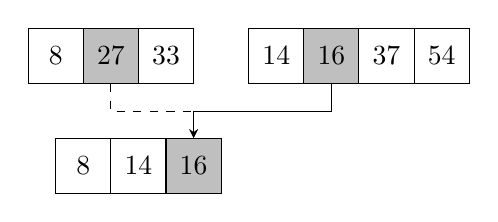
\begin{tikzpicture}[>=stealth, scale=0.7]
\tikzstyle{every node}=[draw,minimum size =7mm,fill=white]
\node[rectangle](l20) at (0,-4) {8};
\node[rectangle,fill=lightgray](l21) at (1,-4) {27};
\node[rectangle](l22) at (2,-4) {33};
\node[rectangle](l23) at (4,-4) {14};
\node[rectangle,fill=lightgray](l24) at (5,-4) {16};
\node[rectangle](l25) at (6,-4) {37};
\node[rectangle](l26) at (7,-4) {54};
\node[rectangle](t20) at (0.5,-6) {8};
\node[rectangle](t21) at (1.5,-6) {14};
\node[rectangle,fill=lightgray](t22) at (2.5,-6) {16};
\draw[->] (l24.south) -- +(0,-0.5) -|  (t22.north);
\draw[->,dashed] (l21.south) -- +(0,-0.5) -|  (t22.north);
\end{tikzpicture}
\end{center}
%--------------------------------------------------------------------------
\vskip 4mm
%--------------------------------------------------------------------------
\begin{center}
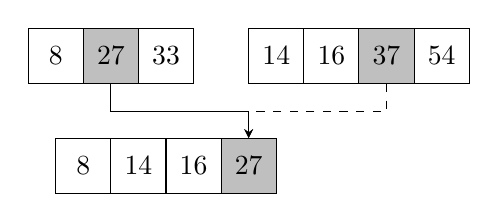
\begin{tikzpicture}[>=stealth, scale=0.7]
\tikzstyle{every node}=[draw,minimum size =7mm,fill=white]
\node[rectangle](l30) at (0,-8) {8};
\node[rectangle,fill=lightgray](l31) at (1,-8) {27};
\node[rectangle](l32) at (2,-8) {33};
\node[rectangle](l33) at (4,-8) {14};
\node[rectangle](l34) at (5,-8) {16};
\node[rectangle,fill=lightgray](l35) at (6,-8) {37};
\node[rectangle](l36) at (7,-8) {54};
\node[rectangle](t30) at (0.5,-10) {8};
\node[rectangle](t31) at (1.5,-10) {14};
\node[rectangle](t32) at (2.5,-10) {16};
\node[rectangle,fill=lightgray](t33) at (3.5,-10) {27};
\draw[->] (l31.south) -- +(0,-0.5) -| (t33.north);
\draw[->,dashed] (l35.south) -- +(0,-0.5) -|  (t33.north);
\end{tikzpicture}
\end{center}
%--------------------------------------------------------------------------
\vskip 4mm
%--------------------------------------------------------------------------
\begin{center}
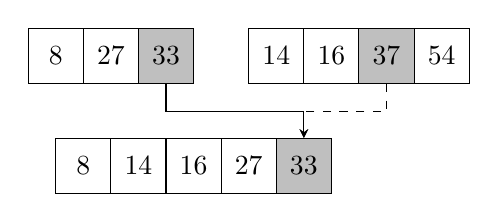
\begin{tikzpicture}[>=stealth, scale=0.7]
\tikzstyle{every node}=[draw,minimum size =7mm,fill=white]
\node[rectangle](l40) at (9,0) {8};
\node[rectangle](l41) at (10,0) {27};
\node[rectangle,fill=lightgray](l42) at (11,0) {33};
\node[rectangle](l43) at (13,0) {14};
\node[rectangle](l44) at (14,0) {16};
\node[rectangle,fill=lightgray](l45) at (15,0) {37};
\node[rectangle](l46) at (16,0) {54};
\node[rectangle](t40) at (9.5,-2) {8};
\node[rectangle](t41) at (10.5,-2) {14};
\node[rectangle](t42) at (11.5,-2) {16};
\node[rectangle](t43) at (12.5,-2) {27};
\node[rectangle,fill=lightgray](t44) at (13.5,-2) {33};
\draw[->,dashed] (l45.south) -- +(0,-0.5) -|  (t44.north);
\draw[->] (l42.south) -- +(0,-0.5) -|  (t44.north);
\end{tikzpicture}
\end{center}
%--------------------------------------------------------------------------
\vskip 4mm
%--------------------------------------------------------------------------
\begin{center}
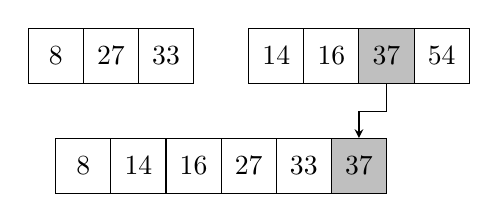
\begin{tikzpicture}[>=stealth, scale=0.7]
\tikzstyle{every node}=[draw,minimum size =7mm,fill=white]
\node[rectangle](l50) at (9,-4) {8};
\node[rectangle](l51) at (10,-4) {27};
\node[rectangle](l52) at (11,-4) {33};
\node[rectangle](l53) at (13,-4) {14};
\node[rectangle](l54) at (14,-4) {16};
\node[rectangle,fill=lightgray](l55) at (15,-4) {37};
\node[rectangle](l56) at (16,-4) {54};
\node[rectangle](t50) at (9.5,-6) {8};
\node[rectangle](t51) at (10.5,-6) {14};
\node[rectangle](t52) at (11.5,-6) {16};
\node[rectangle](t53) at (12.5,-6) {27};
\node[rectangle](t54) at (13.5,-6) {33};
\node[rectangle,fill=lightgray](t55) at (14.5,-6) {37};
\draw[->] (l55.south) -- +(0,-0.5) -|  (t55.north);
\end{tikzpicture}
\end{center}
%--------------------------------------------------------------------------
\vskip 4mm
%--------------------------------------------------------------------------
\begin{center}
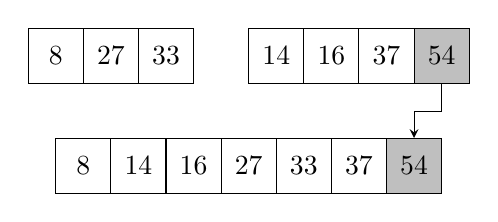
\begin{tikzpicture}[>=stealth, scale=0.7]
\tikzstyle{every node}=[draw,minimum size =7mm,fill=white]
\node[rectangle](l60) at (9,-8) {8};
\node[rectangle](l61) at (10,-8) {27};
\node[rectangle](l62) at (11,-8) {33};
\node[rectangle](l63) at (13,-8) {14};
\node[rectangle](l64) at (14,-8) {16};
\node[rectangle](l65) at (15,-8) {37};
\node[rectangle,fill=lightgray](l66) at (16,-8) {54};
\node[rectangle](t60) at (9.5,-10) {8};
\node[rectangle](t61) at (10.5,-10) {14};
\node[rectangle](t62) at (11.5,-10) {16};
\node[rectangle](t63) at (12.5,-10) {27};
\node[rectangle](t64) at (13.5,-10) {33};
\node[rectangle](t65) at (14.5,-10) {37};
\node[rectangle,fill=lightgray](t66) at (15.5,-10) {54};
\draw[->] (l66.south) -- +(0,-0.5) -| (t66.north);
\end{tikzpicture}
\end{center}
%--------------------------------------------------------------------------
\newpage

%--------------------------------------------------------------------------
%--------------------------------------------------------------------------
\begin{lstlisting}[numbers=left,caption = {Fusion de deux listes triées en une nouvelle liste},label={fn:fusion}]
def fusion(l1,l2):
    """Entree : deux listes
       Requis : les listes sont triées
       Sortie : une liste triée contenant tous 
                les éléments des deux listes initiales"""
    n1 = len(l1)
    n2 = len(l2)
    resultat = []
    pos1 = 0
    pos2 = 0
    while pos1 < n1 and pos2 < n2:
        if plusGrand(l2[pos2],l1[pos1]):
            resultat.append(l1[pos1])
            pos1 = pos1 + 1
        else:
            resultat.append(l2[pos2])
            pos2 = pos2 + 1
    if pos1 == n1:
        return resultat + l2[pos2: n2]
    else:
        return resultat + l1[pos1: n1]
\end{lstlisting}
%--------------------------------------------------------------------------
%--------------------------------------------------------------------------
\begin{itemize}
\item Ligne 8 On initialise la liste à renvoyer.
\item Ligne 9-10 Dans les listes à fusionner  on doit savoir où sont les éléments à comparer. Ces éléments sont indiqués par deux indices de position \type{pos1} et \type{pos2}. Ils indiquent le premier élément non encore placé dans la liste finale. Comme les deux listes sont triées le plus petit élément restant est à l'une de ces deux positions.
\item Ligne 11 On répète autant de fois qu'il y des éléments restant dans les deux listes. 
\item Lignes 12-14 Si le plus petit élément restant est dans la première liste on  l'ajoute au résultat et on incrémente la position du premier élément à comparer.
\item Lignes 15-17 Si le plus petit élément restant est dans la seconde liste on  l'ajoute au résultat.
\item Ligne8 18-21 En sortie de la boucle une des deux liste a été complètement utilisée et on ajoute ce qui reste de l'autre au résultat.
\end{itemize}
%--------------------------------------------------------------------------

On a employé une boucle \type{while}, on peut préférer la sécurité d'une boucle \type{for}
%--------------------------------------------------------------------------
%--------------------------------------------------------------------------
\begin{lstlisting}
def fusion(l1,l2):
    n1 = len(l1)
    n2 = len(l2)
    resultat = [0]*(n1+n2)
    pos1 = 0
    pos2 = 0
    for i in range(n1+n2):
        if pos1 == n1:
            resultat.append(l2[pos2])
            pos2 = pos2 + 1
        elif pos2 == n2:
            resultat.append(l1[pos1])
            pos1 = pos1 + 1
        elif plusGrand(l2[pos2],l1[pos1]):
            resultat.append(l1[pos1])
            pos1 = pos1 + 1
        else:
            resultat.append(l2[pos2])
            pos2 = pos2 + 1
    return resultat
\end{lstlisting}
%--------------------------------------------------------------------------
%--------------------------------------------------------------------------
\subsection{Analyse}
%--------------------------------------------------------------------------
%--------------------------------------------------------------------------
\subsubsection{Terminaison}
%--------------------------------------------------------------------------
\type{fusion} termine car \type{i1+i2} augmente de 1 au moins à chaque étape, on parvient donc à \type{i1 >= n1} ou \type{i2 >= n2} après un nombre fini de passages. Dans le cas d'une boucle \type{for} elle termine naturellement.

La terminaison de la fonction récursive \type{triFusion} se fait par récurrence.

\begin{itemize}
\item Elle termine directement si la liste a moins d'un élément.

\item Si elle termine pour les listes de moins de $n-1$ éléments avec $n\ge 2$, l'appel de la fonction pour une liste de taille $n$ fait appel à la fonction pour des listes de taille $n// 2$ et $n-n//2$.

Pour $n$ pair, $n=2p$ on a $n// 2=n-n//2=p < 2p=n$ car $p$ est non nul pour $n\ge 2$.

Pour $n$ impair, $n=2p+1$ on a $n// 2=p< n-n// 2=p+1<2p+1=n$.

Dans tous les cas les appels récursifs terminent d'après l'hypothèse de récurrence.

Comme \type{fusion} termine on en déduit que \type{triFusion} termine pour les liste de taille $n$.

\item La fonction \type{triFusion} termine pour toutes les listes.
\end{itemize}
%--------------------------------------------------------------------------
\subsubsection{Preuve}
%--------------------------------------------------------------------------
On commence par la preuve de la fusion

On suppose que les listes \type{l1} et \type{l2} sont triées.

Une propriété vérifiée à chaque passage dans la boucle \type{while} est que la liste \type{resultat} est triée et tous ses éléments sont majorés par les éléments de \type{l1[pos1:n1]} et de \type{l2[pos2:n2]}.

On peut alors prouver le tri.

Une liste de taille 0 ou 1  est recopiée et est déjà triée, l'algorithme est correct dans ce cas.

On suppose que la fonction renvoie une liste triée avec les mêmes élément pour toute liste de taille majorée par $n-1$. On considère une liste de taille $n$.

Les listes extraites sont de taille strictement inférieure à $n$ donc les listes \type{l1} et \type{l2} sont triées et contiennent les éléments des deux listes extraites. La preuve de la fusion montre alors que la liste renvoyée est triée et contient tous les éléments de la liste initiale.
%-------------------------------------------------------------------------------
\subsubsection{Complexité}
%--------------------------------------------------------------------------

La complexité est le nombre de comparaisons d'éléments de la liste.

La complexité de la fusion de deux listes de taille respectives $n_1$ et $n_2$ est au plus $n_1+n_2$ car on fait au plus une comparaison pour chaque $i$ dans la boucle (en fait au plus $n_1+n_2-1$).

Lors du tri fusion on sépare en deux listes de tailles respectives $n_1 = n\div 2$ et $n_2 = n-n\div 2$ que l'on trie puis on fusionne les listes triées. 

$n\div p$ désigne la division euclidienne, notée \type{n // p} en Python.

\begin{itemize}
    \item $n_1=n_2 = p$ pour $n$ pair, $n = 2p$,
    \item $n_1=p$, et $n_2 = p+1$ pour $n$ impair, $n = 2p+1$
\end{itemize}

La complexité du tri, $C(n)$, vérifie donc $C(n) \le C(n_1) + C(n_2) +n$.
%--------------------------------------------------------------------------
\begin{thm} [Complexité du tri-fusion]
La complexité du tri fusion d'une liste de taille $n$ en nombre de comparaisons d'éléments vérifie
$C(n) ={\cal O}\bigl(n\log_2(n)\bigr)$.
\end{thm}
%--------------------------------------------------------------------------
{\bf Démonstration} On va montrer par récurrence sur $p$ que $C(n)\le p.2^p$ pour $n \le 2^p$.

Pour $p=0$ cela découle de $C(0)=C(1)=0$.

Si la propriété est vraie pour $p$ on suppose qu'on a $n\le 2^{p+1}$.
\begin{itemize}
    \item Pour $n$ pair, $n_1=n_2 = \frac n2\le 2^p$,
    \item pour $n$ impair on a $n\le 2^{p+1}-1$ et $n_1< n_2 = \frac{n+1}2\le 2^p$.
\end{itemize}

On en déduit, d'après l'hypothèse de récurrence, $C(n_1)\le p2^p$ et $C(n_2)\le p2^p$ d'où

$C(n) \le C(n_1) + C(n_2) +n \le p2^p+p2^p+2^{p+1} = (p+1)2^{p+1}$ : la propriété est vraie pour $p+1$.

\medskip

Si $p$ est choisi tel que $2^{p-1} < n \le 2^p$ on a $2^p\le 2n$ et $p \le 1+\log_2(n)$ d'où
\[C(n) \le \bigl(1+\log_2(n))2n={\cal O}\bigl(n\log_2(n)\bigr)\]
% %--------------------------------------------------------------------------
% %--------------------------------------------------------------------------
% \subsection{Tri en place}
% %--------------------------------------------------------------------------
% %--------------------------------------------------------------------------
% On peut modifier le schéma proposé en introduction en triant une portion de liste plutôt que des listes extraites. Le tri se fera alors en place et demandera moins de listes créées. Cependant on n'échappe pas à la recopie double de tous les éléments à chaque étape. Voir l'exercice \ref{exo:TimFusion} pour une amélioration.

% On choisit ici de définir la fonction auxilliaire à l'intérieur de la fonction principale, cela permet de ne pas donner la liste comme paramètre car elle est définie dans la fonction.
% %----------------------------------------------------------------
% \begin{lstlisting}[caption = Tri fusion en place]
% def triFusion(liste):
%     """Entree : une liste
%       Sortie : une liste triée avec les mêmes éléments"""
%     n = len(liste)
%     def triFusionEntre(i, j):
%         """Entrées : deux indices
%           Sortie : la liste est triée entre i et j (compris)"""
%         if i < j: # Au moins deux points
%             p = (i+j)//2
%             triFusionEntre(i, p)
%             triFusionEntre(p+1, j)
%             fusionInterne(liste, i, j, p)
%     return triFusionEntre(0, n-1)
% \end{lstlisting}
% %--------------------------------------------------------------------------
% \newpage
% %----------------------------------------------------------------
% \begin{lstlisting}[caption = {Fusion de deux parties triées de liste},label={fn:fusion}]
% def fusionInterne(liste, i, j, p):
%     """Entree : une liste et 3 indices  
%       Requis : i <= p < j, la liste est triée entre i et p
%                              et entre p+1 et j
%       Sortie : la liste est triée entre i et j"""
%     n1 = p - i +1
%     n2 = j - p
%     l1 = liste[i: p+1]
%     l2 = liste[p+1: j+1]
%     pos1 = 0
%     pos2 = 0
%     for k in range(i, j+1):
%         if pos1 == n1:
%             liste[k] = l2[pos2]
%             pos2 = pos2 + 1
%         elif pos2 == n2:
%             liste[k] = l1[pos1]
%             pos1 = pos1 + 1
%         elif plusGrand(l2[pos2],l1[pos1]):
%             liste[k] = l1[pos1]
%             pos1 = pos1 + 1
%         else:
%             liste[k] = l2[pos2]
%             pos2 = pos2 + 1
% \end{lstlisting}
% %--------------------------------------------------------------------------
\newpage
%--------------------------------------------------------------------------
%--------------------------------------------------------------------------
\section{Tri pivot (Quicksort)}
%--------------------------------------------------------------------------
%--------------------------------------------------------------------------
%--------------------------------------------------------------------------
Le tri pivot inverse la difficulté : plutôt que fusionner deux sous-listes triées qui viennent d'un découpage arbitraire il découpe la liste selon un {\bf pivot} qui sert de borne pour séparer les éléments selon le pivot : d'un coté les élément plus petits que le pivot, de l'autre les éléments plus grands.

La séparation en deux listes demande donc un travail, par contre l'assemblage des listes triées est immédiat car les éléments de la première sous-liste sont inférieurs aux éléments de la seconde.
%--------------------------------------------------------------------------
%--------------------------------------------------------------------------
\subsection{Écriture du découpage}
%--------------------------------------------------------------------------
%--------------------------------------------------------------------------
Dans le tri fusion on a renvoyé une nouvelle liste (triée) car la fusion en place est ardue.

Pour le tri rapide il est possible de réaliser le tri en place car le découpage peut se faire ainsi.

On doit choisir l'élément qui sert de pivot : nous allons utiliser le dernier élément de la liste à trier mais on pourrait utiliser le premier élément de la liste ou un élément choisi au hasard. Pour ce faire il suffirait d'échanger l'élément choisi et le dernier avant d'appliquer les fonctions ci-dessous.

Comme les sous-listes sont incluses dans la liste de taille $n$, on devra écrire des fonctions intermédiaires qui travaillent sur une portion de la liste, que l'on nommera {\bf segment}. Il faudra inclure deux paramètres qui correspondent au début et à la fin du segment, on choisira les paramètre $a$ et $b$ tels que les indices utilisés sont ceux allant de $a$ à $b$, bornes comprises.

\medskip

On commence par le découpage en deux sous-segments.

On veut transformer un segment de la forme 
%--------------------------------------------------------------------------
\begin{center}
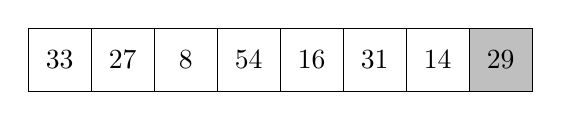
\begin{tikzpicture}[scale=0.8]
\tikzstyle{every node}=[draw,minimum size =8mm,fill=white]
\node[rectangle](l00) at (0,6) {33};
\node[rectangle](l01) at (1,6) {27};
\node[rectangle](l02) at (2,6) {8};
\node[rectangle](l03) at (3,6) {54};
\node[rectangle](l04) at (4,6) {16};
\node[rectangle](l05) at (5,6) {31};
\node[rectangle](l06) at (6,6) {14};
\node[rectangle,fill=lightgray](l06) at (7,6) {29};
\end{tikzpicture} 
\end{center}
%--------------------------------------------------------------------------
en un segment, qui pourrait être
%--------------------------------------------------------------------------
\begin{center}
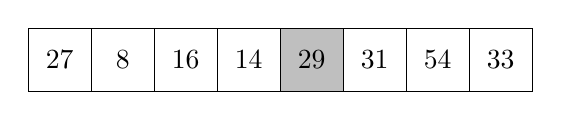
\begin{tikzpicture}[scale=0.8]
\tikzstyle{every node}=[draw,minimum size =8mm,fill=white]
\node[rectangle](l00) at (0,6) {27};
\node[rectangle](l01) at (1,6) {8};
\node[rectangle](l02) at (2,6) {16};
\node[rectangle](l03) at (3,6) {14};
\node[rectangle,fill=lightgray](l04) at (4,6) {29};
\node[rectangle](l05) at (5,6) {31};
\node[rectangle](l06) at (6,6) {54};
\node[rectangle](l06) at (7,6) {33};
\end{tikzpicture} 
\end{center}
%--------------------------------------------------------------------------
On peut remarquer que le pivot est à sa place. En effet les termes placés avant lui sont inférieurs et les termes placés ensuite sont supérieurs.

\medskip

On parcourt la liste entre $a$ et $b-1$ puisque le pivot est en $b$.

On maintient 2 variables d'indice
\begin{itemize}
  \item la première, $i$, est l'indice de la boucle \type{for} qui est la position de l'élément étudié,
  \item la seconde, $k$, est la première position après les termes plus petits que le pivot.
\end{itemize}

On compare chaque terme au pivot.

S'il est plus grand on le laisse en place.
%--------------------------------------------------------------------------
\begin{center}
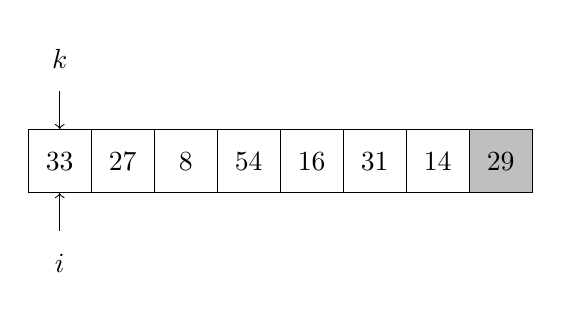
\begin{tikzpicture}[scale=0.8]
\tikzstyle{every node}=[draw,minimum size =8mm,fill=white]
\node[rectangle](l00) at (0,6) {33};
\node[rectangle](l01) at (1,6) {27};
\node[rectangle](l02) at (2,6) {8};
\node[rectangle](l03) at (3,6) {54};
\node[rectangle](l04) at (4,6) {16}; 
\node[rectangle](l05) at (5,6) {31};
\node[rectangle](l06) at (6,6) {14};
\node[rectangle,fill=lightgray](l07) at (7,6) {29};
\draw[<-] (l00.north) -- +(0,0.6) node[draw=none,above]{$k$};
\draw[<-] (l00.south) -- +(0,-0.6) node[draw=none,below]{$i$};
\end{tikzpicture} 
\end{center}
%--------------------------------------------------------------------------
S'il est plus petit, on le permute pour le mettre à la position $k$ puis on incrémente $k$. 
%--------------------------------------------------------------------------
\begin{center}
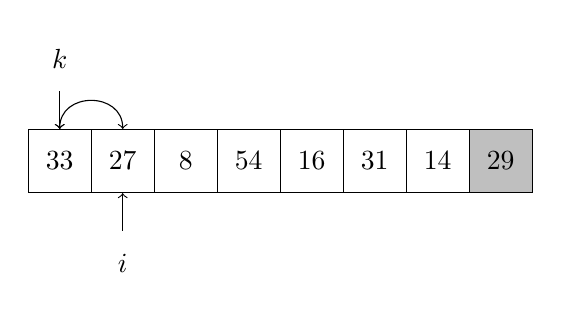
\begin{tikzpicture}[scale=0.8]
\tikzstyle{every node}=[draw,minimum size =8mm,fill=white]
\node[rectangle](l10) at (0,3) {33};
\node[rectangle](l11) at (1,3) {27};
\node[rectangle](l12) at (2,3) {8};
\node[rectangle](l13) at (3,3) {54};
\node[rectangle](l14) at (4,3) {16}; 
\node[rectangle](l15) at (5,3) {31};
\node[rectangle](l16) at (6,3) {14};
\node[rectangle,fill=lightgray](l17) at (7,3) {29};
\draw[<-] (l10.north) -- +(0,0.6) node[draw=none,above]{$k$};
\draw[<-] (l11.south) -- +(0,-0.6) node[draw=none,below]{$i$};
\draw[<->] (l11.north) ..controls +(0,0.6) and +(0,0.6) .. (l10.north);
\end{tikzpicture} 
\end{center}
%--------------------------------------------------------------------------
\begin{center}
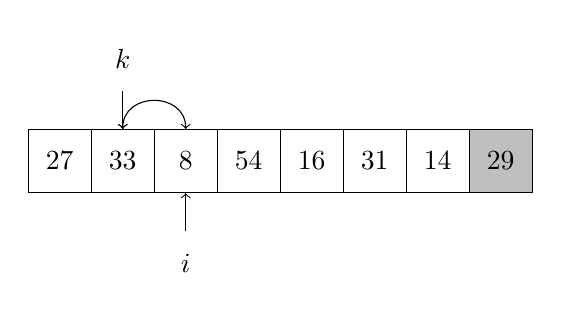
\begin{tikzpicture}[scale=0.8]
\tikzstyle{every node}=[draw,minimum size =8mm,fill=white]
\node[rectangle](l20) at (0,0) {27};
\node[rectangle](l21) at (1,0) {33};
\node[rectangle](l22) at (2,0) {8};
\node[rectangle](l23) at (3,0) {54};
\node[rectangle](l24) at (4,0) {16}; 
\node[rectangle](l25) at (5,0) {31};
\node[rectangle](l26) at (6,0) {14};
\node[rectangle,fill=lightgray](l27) at (7,0) {29};
\draw[<-] (l21.north) -- +(0,0.6) node[draw=none,above]{$k$};
\draw[<-] (l22.south) -- +(0,-0.6) node[draw=none,below]{$i$};
\draw[<->] (l22.north) ..controls +(0,0.6) and +(0,0.6) .. (l21.north);
\end{tikzpicture} 
\end{center}
%--------------------------------------------------------------------------
\begin{center}
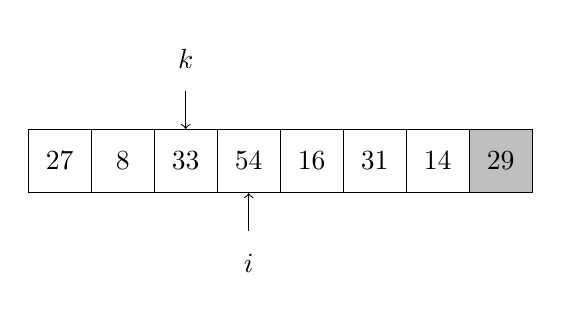
\begin{tikzpicture}[scale=0.8]
\tikzstyle{every node}=[draw,minimum size =8mm,fill=white]
\node[rectangle](l30) at (0,-3) {27};
\node[rectangle](l31) at (1,-3) {8};
\node[rectangle](l32) at (2,-3) {33};
\node[rectangle](l33) at (3,-3) {54};
\node[rectangle](l34) at (4,-3) {16}; 
\node[rectangle](l35) at (5,-3) {31};
\node[rectangle](l36) at (6,-3) {14};
\node[rectangle,fill=lightgray](l37) at (7,-3) {29};
\draw[<-] (l32.north) -- +(0,0.6) node[draw=none,above]{$k$};
\draw[<-] (l33.south) -- +(0,-0.6) node[draw=none,below]{$i$};
\end{tikzpicture} 
\end{center}
%--------------------------------------------------------------------------
\begin{center}
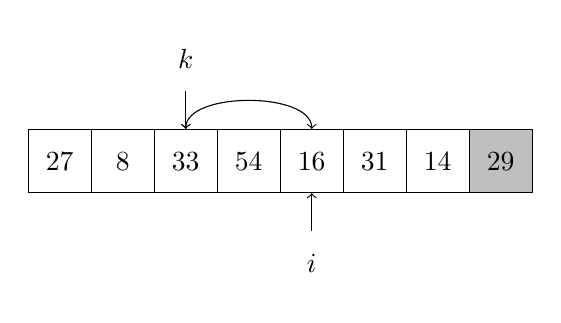
\begin{tikzpicture}[scale=0.8]
\tikzstyle{every node}=[draw,minimum size =8mm,fill=white]
\node[rectangle](l40) at (9,6) {27};
\node[rectangle](l41) at (10,6) {8};
\node[rectangle](l42) at (11,6) {33};
\node[rectangle](l43) at (12,6) {54};
\node[rectangle](l44) at (13,6) {16}; 
\node[rectangle](l45) at (14,6) {31};
\node[rectangle](l47) at (15,6) {14};
\node[rectangle,fill=lightgray](l06) at (16,6) {29};
\draw[<-] (l42.north) -- +(0,0.6) node[draw=none,above]{$k$};
\draw[<-] (l44.south) -- +(0,-0.6) node[draw=none,below]{$i$};
\draw[<->] (l44.north) ..controls +(0,0.6) and +(0,0.6) .. (l42.north);
\end{tikzpicture} 
\end{center}
%--------------------------------------------------------------------------
\begin{center}
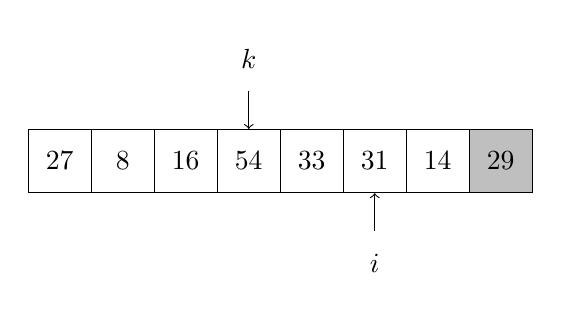
\begin{tikzpicture}[scale=0.8]
\tikzstyle{every node}=[draw,minimum size =8mm,fill=white]

\node[rectangle](l50) at (9,3) {27};
\node[rectangle](l51) at (10,3) {8};
\node[rectangle](l52) at (11,3) {16};
\node[rectangle](l53) at (12,3) {54};
\node[rectangle](l54) at (13,3) {33}; 
\node[rectangle](l55) at (14,3) {31};
\node[rectangle](l56) at (15,3) {14};
\node[rectangle,fill=lightgray](l57) at (16,3) {29};
\draw[<-] (l53.north) -- +(0,0.6) node[draw=none,above]{$k$};
\draw[<-] (l55.south) -- +(0,-0.6) node[draw=none,below]{$i$};
\end{tikzpicture} 
\end{center}
%--------------------------------------------------------------------------
\begin{center}
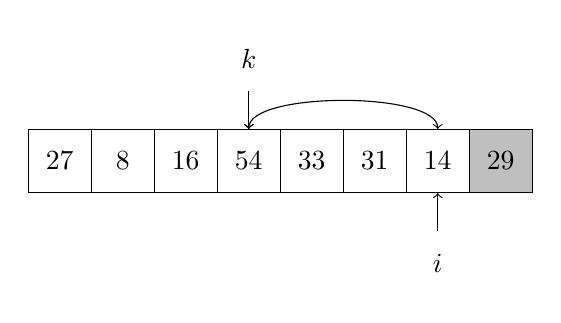
\begin{tikzpicture}[scale=0.8]
\tikzstyle{every node}=[draw,minimum size =8mm,fill=white]
\node[rectangle](l60) at (9,0) {27};
\node[rectangle](l61) at (10,0) {8};
\node[rectangle](l62) at (11,0) {16};
\node[rectangle](l63) at (12,0) {54};
\node[rectangle](l64) at (13,0) {33}; 
\node[rectangle](l65) at (14,0) {31};
\node[rectangle](l66) at (15,0) {14};
\node[rectangle,fill=lightgray](l67) at (16,0) {29};
\draw[<-] (l63.north) -- +(0,0.6) node[draw=none,above]{$k$};
\draw[<-] (l66.south) -- +(0,-0.6) node[draw=none,below]{$i$};
\draw[<->] (l66.north) ..controls +(0,0.6) and +(0,0.6) .. (l63.north);
\end{tikzpicture} 
\end{center}
%--------------------------------------------------------------------------
À la fin on permute le pivot à la position $k$.
%--------------------------------------------------------------------------
\begin{center}
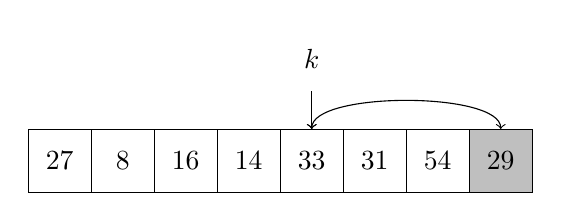
\begin{tikzpicture}[scale=0.8]
\tikzstyle{every node}=[draw,minimum size =8mm,fill=white]
\node[rectangle](l70) at (9,-3) {27};
\node[rectangle](l71) at (10,-3) {8};
\node[rectangle](l72) at (11,-3) {16};
\node[rectangle](l73) at (12,-3) {14};
\node[rectangle](l74) at (13,-3) {33}; 
\node[rectangle](l75) at (14,-3) {31};
\node[rectangle](l76) at (15,-3) {54};
\node[rectangle,fill=lightgray](l77) at (16,-3) {29};
\draw[<-] (l74.north) -- +(0,0.6) node[draw=none,above]{$k$};
\draw[<->] (l77.north) ..controls +(0,0.6) and +(0,0.6) .. (l74.north);
\end{tikzpicture} 
\end{center}
%--------------------------------------------------------------------------
On renverra la position finale du pivot car elle servira à définir les deux segments suivants.

\newpage
Pour permuter deux éléments dans une liste on utilise la fonction classique.
%--------------------------------------------------------------------------
\begin{lstlisting}
def echanger(liste,a,b):
    """Entree : une liste et deux entiers
       Requis : 0 <= a <= b < len(liste)
       Sortie : les valeurs dans la liste
                aux position a et b sont échangées"""
    temp = liste[a]
    liste[a] = liste[b]
    liste[b] = temp
\end{lstlisting}
%--------------------------------------------------------------------------
%--------------------------------------------------------------------------
\begin{lstlisting}[caption = {Découpage pour le tri rapide},label={fn:separe}]
def pivotage(liste,a,b):
    """Entree : une liste et deux entiers
       Requis : 0 <= a <= b < len(liste)
       Sortie : un entier p (a <= p <= b) avec
       le dernier élément placé en p qui sépare
       les élément plus petits et plus grands que lui """
    k = a
    pivot = liste[b]
    for i in range(a, b):
        if plusGrand(pivot, liste[i]):
            echanger(liste, i, k)
            k = k + 1
    echanger(liste, k, b)
    return k
\end{lstlisting}
%--------------------------------------------------------------------------
%--------------------------------------------------------------------------
\subsection{Écriture du tri}
%--------------------------------------------------------------------------
%--------------------------------------------------------------------------
Pour écrire le tri on utilise une fonction auxiliaire, récursive qui trie entre 2 bornes .
%--------------------------------------------------------------------------
\begin{lstlisting}[caption = {Tri rapide}]
def tri_entre(liste, a, b):
    """Entree : une liste et deux entiers
       Requis : 0 <= a <= b < len(liste)
       Sortie : la liste est triee entre a et b"""
    if b > a: 
        p = pivotage(liste, a, b)
        tri_entre(liste, a, p-1)
        tri_entre(liste, p+1, b)
        
def triRapide(liste):
    """Entree : une liste
       Sortie : la liste est triee"""
    n = len(liste)
    tri_entre(liste, 0, n-1)
\end{lstlisting}
%--------------------------------------------------------------------------
\newpage
%--------------------------------------------------------------------------
\subsection{Analyse}
%--------------------------------------------------------------------------
%--------------------------------------------------------------------------
\subsubsection{Terminaison}
%--------------------------------------------------------------------------
\type{pivotage} termine car elle ne fait appel qu'à une boucle \type{for}.

On prouve que la fonction récursive \type{tri\_entre} termine par récurrence sur la longueur de la portion à trier car, lors de chaque appel récursif, celle-ci diminue de 1 au moins.

On en déduit immédiatement que \type{triRapide} termine.
%--------------------------------------------------------------------------
%--------------------------------------------------------------------------
\subsubsection{Preuve}
%--------------------------------------------------------------------------
La fonction de séparation doit produire, à chaque étape, quatre parties :
\begin{enumerate}
\item les éléments plus petits que le pivot, on a choisit une inégalité large,
\item suivis des éléments strictement supérieurs au pivot,
\item les éléments non traités suivent,
\item le pivot est à la dernière position durant la boucle.
\end{enumerate}
On peut alors prouver que les propriétés suivantes forment un invariant.
\[
{\cal P}(i)\left\{
\begin{matrix}
(1)& \hbox{\type{liste[a:k]} est majorée par le pivot}\hfill\\
(2)& \hbox{\type{liste[k:i]} est strictement minorée par le pivot}\\
\end{matrix}
\right.
\]

La preuve du tri s'en déduit.
%--------------------------------------------------------------------------
%--------------------------------------------------------------------------
\subsubsection{Complexité}
%--------------------------------------------------------------------------
%--------------------------------------------------------------------------
\type{pivotage(l,a,b)} fait une comparaison pour chaque $i$ entre $a$ et $b-1$, sa complexité, en nombre de comparaisons, est donc $b-a$.

On note $C(l,a,b)$ le nombre de comparaisons lors de l'appel de \type{tri\_entre(l,a,b)}.

On a donc $C(l,a,b) = b-a+C(l,a,p-1)+C(l,p+1,b)$ si la fonction \type{pivotage} a renvoyé $p$.

\medskip

{\bf Exemple 1} Dans le cas où \type{pivotage(l,a,b)} renvoie $b$ à chaque appel, ce qui est le cas lorsque la liste initiale est déjà triée,  la relation ci-dessus devient

$C(l,a,b) = b-a+C(l,a,b-1)+C(l,b+1,b)= b-a+C(l,a,b-1)$ 

car la complexité pour une liste vide est nulle.

On en déduit qu'alors $C(l,a,b) = b-a+(b-a-1) +\cdots+1$.

En particulier $C(l,0,n-1) = \frac{n(n-1)}2$ : la complexité du tri d'une liste de taille $n$ est un ${\cal O}\bigl(n^2\bigr)$, le tri n'est pas efficace dans ce cas.

\medskip 

{\bf Exemple 2} 

On suppose que $n=2^p-1$ et qu'à chaque étape \type{pivotage(l,a,b)} renvoie un indice situé au milieu, en particulier, s'il y a un nombre impair d'éléments, \type{pivotage(l,a,b)} renvoie $\frac{a+b}2$.

\begin{center}
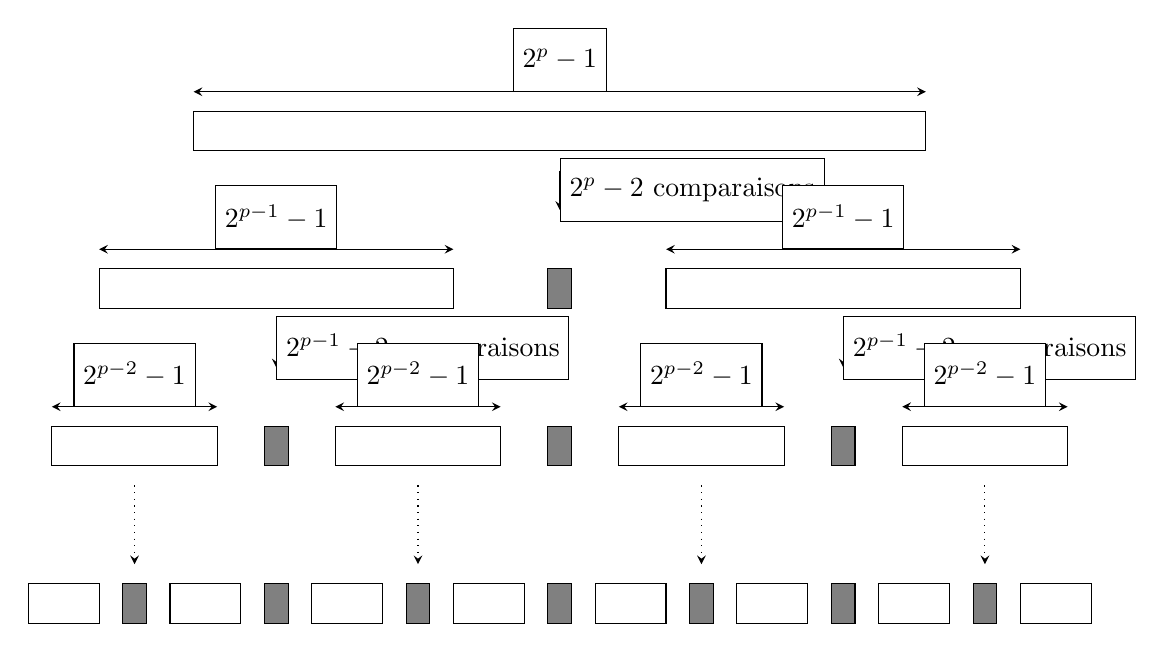
\begin{tikzpicture}[>=stealth, xscale=0.3,yscale=0.5]
\draw[<->] (-15,1.5) -- node[above]{$2^p-1$} +(31,0);
\draw (-15,0) rectangle +(31, 1);
\draw[->] (0.5,-0.5)  -- node[right]{$2^p-2$ comparaisons}+(0,-1);
\foreach\x in {-19, 5} 
 {\draw (\x,-4) rectangle +(15, 1);
  \draw[<->] (\x,-2.5) -- node[above]{$2^{p-1}-1$} +(15,0);
  \draw[->] ({\x+7.5},-4.5)  -- node[right]{$2^{p-1}-2$ comparaisons}+(0,-1);};
\draw[fill = gray](0, -4) rectangle + (1,1);
\foreach\x in {-21, -9, 3, 15} 
 {\draw (\x,-8) rectangle +(7, 1);
  \draw[<->] (\x,-6.5) -- node[above]{$2^{p-2}-1$} +(7,0);
  \draw[dotted,->] ({\x+3.5},-8.5)  -- +(0,-2);};
\foreach\x in {-12, 0, 12} \draw[fill = gray](\x, -8) rectangle + (1,1);
\foreach\x in {-22, -16, -10, -4, 2, 8, 14, 20} \draw (\x,-12) rectangle +(3, 1);
 \foreach\x in {-18, -12, -6, 0, 6, 12, 18} \draw[fill = gray](\x, -12) rectangle + (1,1);

\end{tikzpicture}
\end{center}
À chaque étape on double le nombre de segments et, entre deux segments, il y a un élément qui a été un pivot. Si on note $m_k$ le nombre de segments de taille $2^k-1$, il sont séparés par $m_k-1$ pivots donc on a $2^p-1 = m_k.(2^k-1)+m_k-1 = m_k.2^k - 1$ : on en déduit $m_k=2^{p-k}$.

Ces $m_k$ segments occasionnent chacun $2^k-2$ comparaisons. Le nombre de comparaison est donc 
\begin{align*}
    C(n) 
    &= \sum_{k=2}^p m_k.(2^k-2) = \sum_{k=2}^p 2^{p-k}.(2^k-2) \\
    &= \sum_{k=2}^p \bigl(2^p - 2^{p-k+1}\bigr)
     = \sum_{k=2}^p 2^p - \sum_{k=2}^p 2^{p-k+1}\\
    &= (p-1)2^p - \sum_{i = 1}^{p-1} 2^i
     = (p-1)2^p - \bigl(2^p - 2)
     = (p-2)2^p - 2
\end{align*}
On a $2^p = n+1$ donc $p=\log_2(n+1)$ donc $C(n) = \bigl(\log_2(n+1) -2\bigr)(n+1) + 2$, la complexité est un ${\cal O}\bigl(n\log_2(n)\bigr)$, le tri est efficace dans ce cas.

\medskip

Entre ces deux extrêmes on a le cas moyen : 
%--------------------------------------------------------------------------
\begin{thm} [Complexité moyenne du tri rapide]
La complexité moyenne du tri rapide d'une liste de taille $n$ en nombre de comparaisons d'éléments est un ${\cal O}\bigl(n\log_2(n)\bigr)$.
\end{thm}
%--------------------------------------------------------------------------
%--------------------------------------------------------------------------
Ce résultat doit être connu mais pas sa démonstration.
%--------------------------------------------------------------------------
% \newpage
%--------------------------------------------------------------------------
\subsection{Amélioration}
%--------------------------------------------------------------------------
%--------------------------------------------------------------------------
On va améliorer la fonction \type{pivotage} avec l'introduction d'un choix aléatoire. Cela permettra d'obtenir une complexité qui ne sera pas constante mais dont l'espérance est semblable à la complexité moyenne ci-dessus.

On utilise la fonction \type{randint(a, b)} du module \type{random} qui choisit aléatoirement un entier compris, avec les bornes comprises, entre $a$ et $b$.
%--------------------------------------------------------------------------
\begin{lstlisting}[caption = {Découpage aléatoire pour le tri rapide}]
def pivotage(liste,a,b):
    """Entree : une liste et deux entiers
       Requis : 0 <= a <= b < len(liste)
       Sortie : un entier p (a <= p <= b) avec
       le dernier élément placé en p qui sépare
       les élément plus petits et plus grands que lui """
    p = random.randint(a, b) # on choisit un pivot au hasard
    echanger(liste, p, b)     # on le place à la fin
    pivot = liste[b]         # on continue comme avant
    k = a
    for i in range(a, b):
        if plusGrand(pivot, liste[i]):
            echanger(liste, i, k)
            k = k + 1
    echanger(liste, k, b)
    return k
\end{lstlisting}
%--------------------------------------------------------------------------
La complexité devient maintenant une variable aléatoire $X_C$ dont on cherche à déterminer l'espérance ; c'est le nombre de comparaisons effectuée lors du tri.

On note $a_1< a_2 < \cdots < a_n$ les $n$ éléments, supposés distincts de la liste triée.

Pour calculer l'espérance on utilise la linéarité. Pour cela on définit la variable aléatoire $X_{i,j}$ qui vaut 1 si $a_i$ et $a_j$ sont comparés à un moment dans le tri et 0 si non. 

On a alors $\displaystyle X_C = \sum_{1\le i< j \le n} X_{i, j}$ donc $\displaystyle E(X_C) = \sum_{1\le i< j \le n} E(X_{i, j})$

Pour savoir si $a_i$ et $a_j$ sont comparés, on suit leurs positions dans les parties obtenues par les séparations. Si $a_i$ et $a_j$ sont dans un même segment (ce qui est le cas au début) alors le découpage choisit un pivot $m$. On suppose qu'on a $i< j$ donc $a_i < a_j$.

\begin{itemize}
    \item Si on a $m< a_i$ ou $a_j < m$ alors $a_i$ et $a_j$ ne sont pas comparés et restent dans un même segment après le découpage.
    \item Si on a $a_i < m< a_j$ alors $a_i$ et $a_j$ ne sont pas comparés et sont placés dans des segment distincts : ils ne pourront plus être comparés.
    \item si $a_i=m$ ou $a_j=m$, l'un des deux est le pivot. Les deux éléments sont donc comparés, le pivot sera isolé et l'autre élément appartiendra à un segment, ils ne seront plus comparés.
\end{itemize}
On voit donc que $a_i$ et $a_j$ sont comparés si et seulement si, lors du choix d'un pivot entre $a_i$ et $a_j$, ce pivot vaut $a_i$ ou $a_j$. Il y a donc 2 cas où $X_{i,j}$ vaut 1 parmi les $j-i+1$ cas possible du choix d'un pivot dans $\{a_i,a_{i+1}, \ldots, a_j\}$.

On en déduit qu'on a $\displaystyle E(X_{i, j}) = \frac 2{j-i+1}$. 

On peut donc calculer

\begin{align*}
    E(X_C) 
    &= \sum_{1\le i< j \le n} E(X_{i, j})
     = \sum_{1\le i< j \le n} \frac 2{j-i+1}\\
    &= \sum_{i = 1}^{n-1}\sum_{j = i+1}^n \frac 2{j-i+1} \text{ on pose } k = j-i+1\\
    &= \sum_{i = 1}^{n-1}\sum_{k=2}^{n-i+1} \frac 2k
     = \sum_{k = 2}^n\sum_{i = 1}^{n-k+1} \frac 2k\\
    &= \sum_{k = 2}^n\left(\frac 2k \sum_{i = 1}^{n-k+1} 1\right)
     = \sum_{k = 2}^n \frac 2k (n-k+1)\\
    &= (n+1)\sum_{k = 2}^n \frac 2k - \sum_{k = 2}^n \frac {2k}k
     = 2(n+1)\bigl(H_n-1) - \sum_{k = 2}^n 2\\
    &= 2(n+1)H_n -2(n+1) - 2(n-1)\\ 
    &= 2(n+1)H_n - 4n\\
\end{align*}

On a posé $\displaystyle H_n =\sum_{k=1}^n \frac 1k$ et on sait que $H_n\sim \ln(n)$.

On en déduit que $E(X_C)\sim2n\ln(n)={\cal O}\bigl(n\ln(n)\bigr)$.

On peut donc maintenant espérer une complexité log-linéaire pour le tri de toute liste.

% %--------------------------------------------------------------------------
% %--------------------------------------------------------------------------
% \section{Exercices}
% %--------------------------------------------------------------------------
% %--------------------------------------------------------------------------
% %-------------------------------------------------------------------------------
% \begin{Exercise}[title = {Nombre de comparaisons}]

% On suppose que l'on trie à l'aide de comparaisons une liste de taille $n$.

% Montrer que le nombre de comparaisons à effectuer  est au plus $\frac 12n(n-1)$.

% Montrer que si on a $2^p < n! \le 2^{p+1}$ alors on doit avoir effectuer au moins $p+1$ comparaisons pour pouvoir trier toutes les listes de taille $n$.
% \end{Exercise} 
% %-------------------------------------------------------------------------------
% \begin{Answer} Le nombre de couples d'éléments dans un ensemble de $n$ éléments est $\binom n 2 = \frac 12n(n-1)$ : c'est le nombre maximal de comparaisons distinctes que l'on peut faire.

% Il y a $n!$ listes possibles avec $n$ éléments distincts. Le tris de chacune de ces listes doivent être distincts donc les comparaisons doivent permettre de les distinguer. $k$ comparaisons permettent de distinguer $2^k$ cas donc il faut au moins $p+1$ comparaisons pour distinguer tous les désordres possibles.

% On remarquera que l'équivalent $\ln(n!) \sim n\ln(n)$ donne $p \sim K n \ln(n)$ : les complexités en ${\cal O}\bigl(n\log_2(n)\bigr)$. sont optimales.
% \end{Answer}
% %--------------------------------------------------------------------------
% %-------------------------------------------------------------------------------

% \medskip
% %-------------------------------------------------------------------------------
% \def\flr #1{\bigl\lfloor #1 \bigr\rfloor}
% \def\cl #1{\bigl\lceil #1 \bigr\rceil}
% %-------------------------------------------------------------------------------
% Rappel : la fonction \type{floor}, ou partie entière, est définie par la propriété que $\lfloor x \rfloor$ est le plus grand entier inférieur ou égal à $x$.


% On définit de même la fonction \type{ceil} : $\lceil x \rceil$ est le plus petit entier supérieur ou égal à $x$.
% \[
% n = \flr x \iff \left\{\begin{matrix}n\in \Z\cr n\le x < n+1\\ \end{matrix}\right.
% \qquad
% n = \cl x \iff \left\{\begin{matrix}n\in \Z\cr n-1 < x \le n\\ \end{matrix}\right.
% \]
% %--------------------------------------------------------------------------
% %-------------------------------------------------------------------------------
% \begin{Exercise}[title = {Fonctions \type{floor} et \type{ceil}}]
% \begin{enumerate}
% \item  Prouver que $\cl x = 1 + \flr x$ si $x$ appartient à $\R\setminus \Z$.

% Que se passe-t-il pour $x\in \Z$ ?

% \item Prouver que, pour tout $n\in \Z$, $\flr{\frac n2} = n//2$ et 
% $\flr{\frac n2} + \cl{\frac n2} = n$.

% $\flr{\frac n2}$ et $\cl{\frac n2}$ sont donc les cardinaux des sous-listes dans le tri-fusion.

% \item Prouver que, pour tout $n\in \Z$, 
% $\flr{\frac {n+1}2} = \cl{\frac n2}$ et 
% $\cl{\frac {n+1}2} = \flr{\frac n2}+1$
% \end{enumerate}
% \end{Exercise} 
% %-------------------------------------------------------------------------------
% \begin{Answer}
% \begin{enumerate}
%  \item Si $x$ n'est pas entier et  $n\le x < n+1$ pour $n\in \Z$ alors $n< x < n+1$ 
 
%  d'où $n=\flr x$ et $n+1=\cl x$.  
% Pour $n$ entier $\flr n = \cl n = n$.
 
% \item Pour $n$ pair, $n=2p$, $\flr{\frac n2} = \flr p = p =n//2$ et
% $\cl {\frac n2} = \cl p = p = n - n//2$.

% Pour $n$ impair, $n=2p+1$, $\flr{\frac n2} = \flr{p + \frac 12} = p = n//2$ 

% et $\cl {\frac n2} = \cl{p + \frac 12} = p+1 = n - n//2$.
 
% \item Pour $n$ pair, $n=2p$, $\flr{\frac n2} = \cl {\frac n2} = p$ et $\flr{\frac {n+1}2} =p$, 
% $\cl{\frac {n+1}2}=p+1$.

% Pour $n$ impair, $n=2p+1$, $\flr{\frac n2} = p$, $\cl{\frac n2} = p +1$ et
% $\flr{\frac {n+1}2} =\cl{\frac {n+1}2}=p+1$
% \end{enumerate}
% \end{Answer}
% %--------------------------------------------------------------------------
% %-------------------------------------------------------------------------------
% \begin{Exercise}[title = {Invariant de boucle pour la fusion}, label= exo:invFusion]
% Prouver que l'ensemble des propriétés suivantes est un invariant de boucle dans la fonction \type{fusion} (programme \ref{fn:fusion}, page \pageref{fn:fusion})
% \[
% {\cal P}(i)\ 
% \left\{
% \begin{matrix}
% (1)& \hbox{\type{pos1 <= n1}} \hfill\cr
% (2)& \hbox{\type{pos2 <= n2}} \hfill\cr
% (3)& \hbox{\type{pos1 + pos2 = i}} \hfill\cr
% (4)& \hbox{\type{resultat + l1[pos1:n1]} est triée} \hfill\cr
% (5)& \hbox{\type{resultat + l2[pos2:n2]} est triée} \hfill\cr
% (6)& \hbox{\type{resultat + l1[pos1:n1] + l2[pos2:n2]} est une permutation de \type{l1 + l2}}
% \end{matrix}
% \right.
% \]
% \end{Exercise} 
% %-------------------------------------------------------------------------------
% \begin{Answer}
% \begin{itemize}
% \item Au départ \type{resultat} est vide \type{l1} et \type{l2} sont triées et \type{i = pos1 = pos2 = 0} 

% donc les propriétés sont vraies.
% %-------------------------------------------------------------------------------
% \item  On suppose que ces propriétés sont vraies au départ d'un passage de boucle avec 

% \type{i < n1 + n2} ; on effectue alors la boucle. 

% On notera \type{pos1'}, \type{pos2'} et \type{resultat'} les valeurs des variables après la boucle, 

% on note aussi \type{i' = i+1}.

% On suppose qu'on a ajouté \type{l1[pos1]} à la liste \type{resultat}.

% Cela ne peut pas se produire pour \type{pos1 == n1}, traité à la ligne 12 : on a \type{pos1 < n1}.  
 
% On a alors \type{pos1' = pos1 + 1 < n1 + 1} donc  \type{pos1' <= n1}, ce qui donne $(1)$.
 
% La conservation \type{pos2' = pos2} donne $(2)$.

% \type{pos1' + pos2' = pos1 + 1 + pos2 = i + 1 = i'}, ce qui donne $(3)$.

% \type{resultat' = resultat + [a]} et \type{l1[pos1:n1] = [a] + l1[pos1':n1]} donc 

% \type{resultat' + l1[pos1':n1] =  resultat + l1[pos1:n1]}, la propriété $(4)$ reste vraie.

% Comme on a \type{l2[pos2':n2] =  l2[pos2:n2}, la propriété $(6)$ reste vraie aussi.

% \type{l1[pos1]} minore \type{l2[pos2]} donc 
% le dernier terme de \type{resultat'} minore le premier terme de \type{l2[pos2':n2]},

% \type{resultat'} est triée d'après la conservation de (4)

% et \type{l2[pos2':n2]} est triée car extraite d'une liste triée.

% On en déduit que $(5)$ est vérifié.
% \medskip

% On conclut de même si \type{a = l2[pos2]}.

% Ainsi, si ${\cal P}(i)$ est valide au départ de la boucle pour $i$, ${\cal P}(i+1)$ est valide à la fin de la boucle.
% %-------------------------------------------------------------------------------
% \item Pour $i = n1+n2$, les 3 premières conditions imposent \type{pos1 = n1} et \type{pos2 = n2}.

% La condition $(4)$ ou $(5)$ montre que \type{resultat} est triée et la condition $(6)$ indique que cette liste contient tous les éléments. Ainsi le résultat est bien la fusion triée des deux listes.
% \end{itemize}

% On a bien un invariant de boucle qui prouve le résultat attendu.
% \end{Answer}
% %--------------------------------------------------------------------------
% %--------------------------------------------------------------------------
% \begin{Exercise}[title = {Complexité maximale du tri-fusion}]

% On a vu que le le nombre maximal de comparaisons nécessaire dans le tri-fusion une liste de $n$ éléments, $C(n)$, vérifie $C_0=C_1=0$ et 
%  $C_n=C_{\flr {\frac n2}}+C_{\cl {\frac n2}}+n-1$.

% \begin{enumerate}
%  \item On pose $D_n=C_{n+1}-C_n$. 
% Prouver que $D_n=D_{\flr{\frac n2}}+1$ avec $D_0=0$.

% \item En déduire que $D(n)=p+1$ pour $n$ tel que  $2^p \le n < 2^{p+1}$. On notera $p=L(n)$.

% \item Conclure que $C_n=nL(n)+n+1-2^{L(n)+1}$ pour $n\ge 1$.
% \end{enumerate}
% \end{Exercise} 
% %-------------------------------------------------------------------------------
% \begin{Answer}
% \begin{enumerate}
% \item $D_n=C_{n+1}-C_n=C_{\flr{\frac {n+1}2}}+C_{\cl{\frac {n+1}2}}+(n+1)-1
% -\left(C_{\flr{\frac n2}}+C_{\cl{\frac n2}}+n-1\right)$.
 
% En utilisant l'exercice ci-dessus on obtient 

% $D_n=C_{\flr{\frac n2}+1}-C_{\flr{\frac n2}}-1=D_{\flr{\frac n2}}+1$.
% $D_0 = C_1 - C_0=0$

% \item $C_2 = C_1+C_1+1=1$ donc $D_1 = C_2-C_1 = 1$.

% $2^k \le n < 2^{k+1}$ implique $2^{k-1} \le n/2 < 2^{k}$ donc $L(\flr n2) = L(n)-1$.

% On a ainsi $D_n-L(n)=D_{\flr{\frac n2}}+1-\bigl(L(\flr n2)+1\bigr) = D_{\flr{\frac n2}} -L(\flr n2)$ : la suite des différence est constante. En divisant par 2 on aboutit à 1 donc
% $D_n-L(n)=D_1-L()=1$.

% \item On a $C_1=0=L(1)=1.L(1)+1+1-2^{0+1}$ : la propriété est vraie pour $n=0$.

% On suppose que $C_n=nL(n)+n+1-2^{L(n)+1}$ alors

% $C_{n+1}=D(n)+C_n=L(n)+1+C_n=(n+1)L(n)+n+2-2^{L(n)+1}$.

% \medskip

% Si on a $2^p\le n < 2^{p+1}-2$ alors $2^p < n < 2^{p+1}-1$ donc $L(n)=L(n+1)=p$ et on a bien 
% $C_{n+1}=(n+1)L(n+1)+(n+1)+1-2^{L(n+1)+1}$.

% \medskip

% Pour $n=2^{p+1}-1$ alors $n+1=2^{p+1}$ donc $L(n)=p$ et $L(n+1)=p+1$.

% On a aussi $n+1=2^{L(n+1)}$ d'où

% \begin{align*}
% C_{n+1}
% &
% =(n+1)\bigl(L(n+1)-1\bigr)+(n+1)+1-2^{L(n+1)}
% \\ &
% =(n+1)L(n+1)+(n+1)+1-2^{L(n+1)}-(n+1)
% \\&
% =(n+1)L(n+1)+(n+1)+1-2.2^{L(n+1)}
% \\ &
% =(n+1)L(n+1)+(n+1)+1-2^{L(n+1)+1}
% \end{align*}

% \medskip

% Dans les deux cas la formule est vraie pour $n+1$.

% On a démontré la propriété par récurrence.
% \end{enumerate}
% \end{Answer}
% %--------------------------------------------------------------------------
% %--------------------------------------------------------------------------
% \begin{Exercise}[title = {Déplacements partiels dans la fusion en place}]

% Dans le tri fusion en place la fonction de fusion copie tous les éléments dans deux nouvelles listes avant de les replacer dans la liste initiale.

% En fait il est possible de garder la portion de liste de droite en mémoire et d'effectuer la fusion. Écrire une fonction \type{fusion\_gauche} qui effectue ainsi la fusion.

% En remplissant la portion de liste depuis la droite on peut aussi ne copier que la partie droite : écrire une fonction \type{fusion\_droite} qui correspond.
% \end{Exercise} 
% %-------------------------------------------------------------------------------
% \begin{Answer}
% On modifie la fusion en place. 
% \begin{lstlisting}
% def fusion_gauche(liste, i, j, p):
%     """Entree : une liste et 3 indices  
%       Requis : i <= p < j, la liste est triée entre i et p
%                              et entre p+1 et j
%       Sortie : la liste est triée entre i et j"""
%     n1 = p - i +1
%     l1 = liste[i: p+1]
%     pos1 = 0
%     pos2 = p+1
%     for k in range(i, j+1):
%         if pos1 == n1:
%             liste[k] = liste[pos2]
%             pos2 = pos2 + 1
%         elif pos2 == j+1:
%             liste[k] = l1[pos1]
%             pos1 = pos1 + 1
%         elif plusGrand(liste[pos2],l1[pos1]):
%             liste[k] = l1[pos1]
%             pos1 = pos1 + 1
%         else:
%             liste[k] = liste[pos2]
%             pos2 = pos2 + 1   
% \end{lstlisting}

% \newpage
% On remplit les positions depuis la droite. On place le plus grand élément restant à placer.
% \begin{lstlisting}
% def fusion_droite(liste, i, j, p):
%     """Entree : une liste et 3 indices  
%       Requis : i <= p < j, la liste est triée entre i et p
%                              et entre p+1 et j
%       Sortie : la liste est triée entre i et j"""
%     l2 = liste[p+1:j+1]
%     pos1 = p
%     pos2 = j -p -1
%     for k in range(j, i-1, -1):
%         if pos1 == i-1:
%             liste[k] = l2[pos2]
%             pos2 = pos2 - 1
%         elif pos2 == -1:
%             liste[k] = liste[pos1]
%             pos1 = pos1 - 1
%         elif plusGrand(liste[pos1],l2[pos2]):
%             liste[k] = liste[pos1]
%             pos1 = pos1 - 1   
%         else:
%             liste[k] = l2[pos2]
%             pos2 = pos2 - 1
% \end{lstlisting}
% \end{Answer}
% %--------------------------------------------------------------------------
% %--------------------------------------------------------------------------
% \begin{Exercise}[title = {Améliorations de la fusion en place}, label = exo:TimFusion]

% Dans la pratique il arrive que les listes à trier soient partiellement triées. 
% Les améliorations proposées ici sont destinées à diminuer le nombre de comparaisons effectuées dans le cas de listes peu désordonnées. Ces améliorations sont employées dans le tri \Type{TimSort} de python dû à Tim Peters.

% Dans l'exercice précédent on peut remarquer que les éléments les plus grands de la partie de droite (resp. les éléments les plus petits de la partie de gauche) sont laissés en place lors de l'appel à \type{fusion\_gauche} (resp. de  \type{fusion\_droite}). On va tenir compte de cette possibilité.

% On considère l'appel de \type{fusionInterne(liste, i, p, j)} avec $i \le p < j$.

% \begin{enumerate}
%   \item Si on a \type{liste[p] <= liste[p+1]} les deux parties forment déjà une liste triée.
%   \item Si on a \type{liste[p] > liste[p+1]} alors on considère le plus grand entier $k \in \{p+1, p+2, \ldots, j\}$, noté $j_1$, tel que \type{liste[p] > liste[k]}. Les éléments de la liste entre les indices $j_1+1$ et $j$ sont tous plus grands que ceux de la première partie donc sont à leur place.
  
%   De même, si $i_1 = \text{min}\bigl\{k\ ;\ i \le k \le p,\ \type{liste[k] > liste[p+1]}\bigr\}$, les éléments d'indices $i$ à $i_1-1$ sont à leur place. 
  
%   \item Il reste alors à fusionner les parties entre $i_1$ et $p$ à gauche et entre $p+1$ et $j_1$ à droite. Pour minimiser les copies on utilisera \type{fusion\_gauche} ou \type{fusion\_droite} selon les tailles des deux parties.
% \end{enumerate}
% \begin{center}
% \begin{tikzpicture}[scale=0.8]
% \tikzstyle{every node}=[draw,minimum size =8mm,fill=white]
% \foreach \i/\x in {0/4, 1/12, 2/14, 3/15, 4/20, 5/9, 6/13, 7/17, 8/21, 9/24, 10/30}
%   \node[rectangle](l\i) at (\i,0) {\x};
% \draw[<-] (l0.north) -- +(0,0.6) node[draw=none,above]{$i$};
% \draw[<-] (l1.north) -- +(0,0.6) node[draw=none,above]{$i_1$};
% \draw[<-] (l4.north) -- +(0,0.6) node[draw=none,above]{$p$};
% \draw[<-] (l5.north) -- +(0,0.6) node[draw=none,above]{$p+1$};
% \draw[<-] (l7.north) -- +(0,0.6) node[draw=none,above]{$j_1$};
% \draw[<-] (l10.north) -- +(0,0.6) node[draw=none,above]{$j$};
% \end{tikzpicture} 
% \end{center}

% Dans cet exemple on effectue \type{fusion\_droite(liste, i1, p, j1)}.

% \medskip

% Après avoir écrit les fonctions de recherche pour $i_1$ et $j_1$ en utilisant la méthode de dichotomie, écrire la fonction \type{fusionInterne} correspondante.
% \end{Exercise} 
% %-------------------------------------------------------------------------------
% \begin{Answer}
% \begin{lstlisting}
% def plus_petit_majorant(liste, i, j, x):
%     """Entree : une liste et 2 indices et un terme 
%       Requis : la liste est triée entre i et j, liste[j] > x
%       Sortie : le plus petit indice k entre i et j
%                 tel que liste[k] > x"""
%     if i == j:
%         return i
%     else:
%         p = (i+j)//2
%         if plusGrand(liste[p], x):
%             return plus_petit_majorant(liste, i, p, x) 
%         else:
%             return plus_petit_majorant(liste, p+1, j, x)   
% \end{lstlisting}
% \begin{lstlisting}
% def plus_grand_minorant(liste, i, j, x):
%     """Entree : une liste et 2 indices et un terme
%       Requis : la liste est triée entre i et j, liste[i] < x
%       Sortie : le plus grand indice k entre i et j
%                 tel que liste[k] < x"""
%     if i == j:
%         return i
%     else:
%         p = (i+j)//2
%         if plusGrand(x, liste[p+1]):
%             return plus_grand_minorant(liste, p+1, j, x) 
%         else:
%             return plus_grand_minorant(liste, i, p, x)   
% \end{lstlisting}

% \newpage

% \begin{lstlisting}
% def fusionInterne(liste, i, j, p):
%     """Entree : une liste et 3 indices  
%       Requis : i <= p < j, la liste est triée entre i et p
%                              et entre p+1 et j
%       Sortie : la liste est triée entre i et j"""
%     if plusGrand(liste[p], liste[p+1]):
%         i1 = plus_petit_majorant(liste, i, p, liste[p+1])
%         j1 = plus_grand_minorant(liste, p+1, j, liste[p])
%         if j1 - p > p - i1:
%             fusion_gauche(liste, i1, j1, p)
%         else:
%             fusion_droite(liste, i1, j1, p)
% \end{lstlisting}
% \end{Answer}
% %-------------------------------------------------------------------------------
% %-------------------------------------------------------------------------------
% \begin{Exercise}[title = {Tri fusion itératif}]
% Pour réaliser le tri fusion on peut opérer de manière itérative.

% On fusionne les partie de liste de taille 1 deux par deux : on obtient des parties de taille 2 triées.

% On fusionne ces parties pour obtenir des parties de taille 4 triées.

% On recommence ainsi jusqu'à obtenir une liste triée.

% Le travail n'est pas aussi simple car il peut y avoir des résidus de taille plus petite.

% Exemple, pour \type{[2, 15, 22, 8, 37, 17, 28, 5, 12, 31, 23]}, de taille 11.

% \begin{center}
% \begin{tikzpicture}[scale=0.8]
% \tikzstyle{every node}=[draw,minimum size =8mm,fill=white]
% \foreach \x/\d in {2/0, 15/1.5, 22/3.5, 8/5, 37/7, 17/8.5, 28/10.5, 5/12, 12/14, 31/15.5, 10/17.5}
%   \node[rectangle] at (\d,0) {\x};

% \foreach \x/\d in {2/0, 15/1, 8/2.5, 22/3.5, 17/5.5, 37/6.5, 5/8, 28/9, 12/11, 31/12, 10/13.5}
%   \node[rectangle] at (\d,-1.5) {\x};

% \foreach \x/\d in {2/0, 8/1, 15/2, 22/3, 5/4.5, 17/5.5, 28/6.5, 37/7.5, 10/9.5, 12/10.5, 31/11.5}
%   \node[rectangle] at (\d,-3) {\x};

% \foreach \x/\d in {2/0, 5/1, 8/2, 15/3, 17/4, 22/5, 28/6, 37/7, 10/8.5, 12/9.5, 31/10.5}
%   \node[rectangle] at (\d,-4.5) {\x};

% \foreach \x/\d in {2/0, 5/1, 8/2, 10/3, 12/4, 15/5, 17/6, 22/7, 28/8, 31/9, 37/10}
%   \node[rectangle] at (\d,-6) {\x};
% \end{tikzpicture} 
% \end{center}

% Écrire la fonction correspondante.

% \end{Exercise} 
% %-------------------------------------------------------------------------------
% \begin{Answer}
% \begin{lstlisting}
% def triFusion(liste):
%     """Entree : une liste 
%       Sortie : la liste est triée"""
%     n = len(liste)
%     p = 1
%     while p < n:
%         m = n//(2*p)
%         for k in range(m):
%             i = 2*p*k
%             fusionInterne(liste, i, i+2*p-1, i+p-1)
%         if 2*p*m + p < n:
%             fusionInterne(liste, 2*p*m, n-1, 2*p*m+p-1)
%         p = 2*p        
% \end{lstlisting}
% \end{Answer}
% %-------------------------------------------------------------------------------
% %-------------------------------------------------------------------------------
% \begin{Exercise}[title = {Invariant de boucle pour la séparation du tri rapide}, label= exo:invSepare]
% Prouver que l'ensemble des propriétés suivantes est un invariant de boucle dans la fonction \type{pivotage} (programme \ref{fn:separe}, page \pageref{fn:separe})
% \[
% {\cal P}(i)\left\{
% \begin{matrix}
% (1)& \hbox{\type{liste[a:k]} est majorée par le pivot}\hfill\cr
% (2)& \hbox{\type{liste[k:i]} est strictement minorée par le pivot}\cr
% \end{matrix}
% \right.
% \]
% \end{Exercise} 
% %-------------------------------------------------------------------------------
% \begin{Answer}

% Au début du programme on a $k = i=a$ donc ${\cal P}(a)$ ne contient aucune condition : il est vérifié.

% On suppose que ${\cal P}(i)$ est valide au début de la boucle d'indice $i$ avec $i < b-1$.

% \begin{enumerate}
% \item Si le pivot est plus grand que \type{liste[i]} on échange les termes d'indices $i$ et $k$ puis on incrémente $k$, on note $k'$ la nouvelle valeur de $k$ ($k'=k+1$). 
% \type{liste[a:k']} est toujours majorée par le pivot car on a ajouté un terme qui vérifie la condition.

% \type{liste[k':i+1]} comporte les mêmes termes (dans un ordre différent) que l'ancienne liste \type{liste[k:i]} donc est encore minorée par le pivot.
% ${\cal P}(i+1)$ est encore valide dans ce cas.

% \item Si \type{liste[i]} majore le pivot alors \type{liste[a:k]} est inchangée et \type{liste[k:i+1]} contient un élément de plus que \type{liste[k:i]} et ce terme est strictement minoré par le pivot aussi.

% ${\cal P}(i+1)$ est valide aussi dans ce cas.
% \end{enumerate}

% Ainsi ${\cal P}(b-1)$ est vérifié donc tous les éléments d'indices $a$ à $k-1$ sont majorés par le pivot et tous ceux d'indices $k$ à $b-1$ sont minorés strictement par le pivot.

% L'échange des termes d'indices $k$ et $b$ montre que l'indice renvoyé, $k$, est compris entre $a$ et $b$ et sépare la liste selon la comparaison au terme \type{liste[k]}.
% \end{Answer}
% %-------------------------------------------------------------------------------
% %-------------------------------------------------------------------------------
% \begin{Exercise}[title = {Preuve du tri rapide}, label= exo:preuveQS]

% Prouver que le tri rapide trie la liste passée en paramètre.
% \end{Exercise} 
% %-------------------------------------------------------------------------------
% \begin{Answer}

% On prouve que la fonction \type{tri_entre} trie le segment par récurrence sur $b-a$.

% \begin{itemize}
%   \item Si $b-a \le 0$ le segment est vide ou a un seul élément et il est inchangé. 

% Comme toute liste de 0 ou 1 élément est triée, l'algorithme est correct dans ce cas.

% \item On suppose que la fonction \type{tri_entre(liste, i, j)} trie le segment en conservant les élément pour tous $i$ et $i$ tels que $j - i \le m$. On considère un segment de $a$ à $b$ avec $b-a = m+1$.

% La valeur $p$ renvoyé par \type{pivotage} est comprise entre $a$ et $b$.

% On a alors $(b-1)-a \le m$ et $b - (p+1) \le m$ donc l'hypothèse de récurrence affirme que les segments de $a$ à $p-1$ et de $p+1$ à $b$ sont triés après les appels récursifs à la fonction \type{tri_entre}.

% Dans le segment entre $a$ et $b$ on a donc 
% des éléments majorés par \type{liste[p]} entre $a$ et $p-1$,
% suivis de \type{liste[p]} puis suivis par des élément strictement supérieurs : le segment total est trié.

% Comme on a modifié la liste uniquement par des échanges, la liste a les mêmes éléments.
% \end{itemize}

% La fonction \type{tri_entre} renvoie bien la liste permutée dans l'ordre entre $a$ et $b$ pour toute paire d'indices valides donc, en particulier, pour $a=0$ et $b = n-1$ : \type{triRapide} est prouvée.
% \end{Answer}
% %--------------------------------------------------------------------------
% %-------------------------------------------------------------------------------
% \begin{Exercise}[title = {Complexité maximale du tri rapide}]

% Prouver que la complexité du tri rapide d'une liste de taille $n$, en nombre de comparaisons, est majorée par $\frac{n(n-1)}2$.
% \end{Exercise} 
% %-------------------------------------------------------------------------------
% \begin{Answer}
% La complexité du tri d'une liste de taille 1 est 0.

% On a établi que la complexité du tri rapide d'une liste entre $a$ et $b$, $C(a,b)$, vérifie 

% $C(a,b) = b-a+C(a,p-1)+C(p+1,b)$ où $p$ est la position du pivot. 

% On remarque que la complexité ne dépend que de la largeur de l'intervalle donc on peut noter $C(a,b)=C'(n)$ avec $n = b-a+1$. 

% La relation ci-dessus peut s'écrire $C'(n)=n-1 + C'(n_1)+C'(n_2)$ avec $n_1 = p-1-a+1=p-a$ et $n_2=b-(p+1)+1=p-b$ donc $n_1+n_2=n-1$.

% On aboutit ainsi à $C'(n)=n-1 + C'(n_1)+C'(n-1-n_1)$ avec $0\le n_1 \le n-1$ et $C'(1)=0$

% Si on suppose, par récurrence, que $C'(k) \le  \frac{k(k-1)}2$ pour $k < n$ on a 

% $C'(n)\le n-1 + \frac{n_1(n_1-1)}2 + \frac{(n-n_1-1)(n-n_1-2)}2
% =\frac{n(n-1)}2+n_1(n_1-n+1)$.

% Or $n_1\ge 0$ et $n-1-n_1\ge 0$ d'o\`u $n_1(n_1-n+1)\le 0$ puis $C'(n)\le \frac{n(n-1)}2$.

% Le résultat est prouvé par récurrence.
% \end{Answer}
% %--------------------------------------------------------------------------
% %-------------------------------------------------------------------------------
% \begin{Exercise}[title = {Exemples de complexités minimale dans le tri rapide}]

% \type{l3 = [1,3,2,6,5,7,4]} et \type{l4 = [1,3,2,6,5,7,4,12,9,11,10,14,13,15,8]}.

% \begin{enumerate}
% \item  Combien de comparaisons sont effectuées pour trier \type{l3} et \type{l4} ?

% \item Donner un exemple semblable pour une liste de taille 31.

% \item De manière générale comment construire une liste de taille $2^p-1$ telle que les découpages donneront des listes qui seront toujours de taille $2^k-1$ comme dans l'étude du cours ?
% \end{enumerate}
% \end{Exercise} 
% %-------------------------------------------------------------------------------
% \begin{Answer}
% \begin{enumerate}
% \item  10 et 34

% \item \type{L5 = l4 + [24,17,19,18,22,21,23,20,28,25,27,26,30,29,31,16]}

% \item On définit la suites pour $n=2^{p+1}-1$ récursivement.

% On calcule la liste pour $2^p-1$, \type{l}.

% On veut que le découpage selon le pivot $2^p$ donne \type{l} et \type{l1} avec \type{l1}  obtenue en ajoutant $2^p$ à chaque élément : dans ce cas les opérations effectuées sur \type{l} et \type{l1} seront identiques et on est dans le cas de l'étude.

% Si on place les éléments de \type{l} puis ceux de \type{l1} suivis du pivot $2^p$ le parcours du découpage ne changera rien mais on déplace le pivot à sa position donc il faut envoyer le dernier élément de \type{l1} en tête.
% %--------------------------------------------------------------------------
% \begin{lstlisting}
% def listeMin(p):
%     if p <= 1:
%         return [1]
%     else:
%         l1 = listeMin(p-1)
%         pivot = l1[-1]*2
%         l2 = [x+pivot for x in l1]
%         pivot1 = l2.pop()
%         return l1+[pivot1]+l2+[pivot]
% \end{lstlisting}
% %--------------------------------------------------------------------------
% \end{enumerate}
% \end{Answer}
% %--------------------------------------------------------------------------
% %-------------------------------------------------------------------------------
% \begin{Exercise}[title = {Médiane}]
% L'élément médian d'une liste est un élément $p$ de la liste tel que le nombre d'élément de liste inférieurs à $p$ est égal au nombre d'éléments supérieurs (ou à ce nombre -1).

% Par exemple 17 est médian de \type{[5, 27, 12, 33, 17, 8, 18]} 

% \begin{enumerate}
% \item Comment calculer l'élément médian d'une liste de taille $n$ en ${\cal O}\bigl(n\log_2(n)\bigr)$ ?

% \item En adaptant l'algorithme de tri rapide montrer qu'on peut déterminer l'élément médian en temps linéaire en moyenne. L'idée est de généraliser la recherche au $p$-ième élément et de le chercher dans la "bonne sous-liste".
% \end{enumerate}
% \end{Exercise} 
% %-------------------------------------------------------------------------------
% \begin{Answer}
% \begin{enumerate}
% \item On trie la liste, l'élément est le terme d'indice $\flr{\frac n2}$.

% \item Si $p$ est l'indice recherché on sépare la liste. Le pivot se place à l'indice $k$.

% \begin{itemize}
% \item Si $k=p$ on a fini.
% \item Si $k > p$ on cherche l'élément dans la sous-liste de gauche.
% \item Si $k < p$ on cherche l'élément dans la sous-liste de droite.
% \end{itemize}

% \newpage
% %-------------------------------------------------------------------------------
% \begin{lstlisting}
% def auxRech(liste,a,b,p):
%     """Entrées : une liste et 3 entiers
%       Requis : 0 <= a <= p <= b < len(liste)
%       Sortie : la valeur du terme d'indice p dans
%                 la liste triée depuis liste"""
%     if b > a:
%         k = pivotage(liste,a,b)
%         if k == p:
%             return liste[k]
%         elif k > p:
%             return auxRech(liste,a,k-1,p)
%         else:
%             return auxRech(liste,k+1,b,p)
%     else:
%         return liste[a]

% def recherche(l,p):
%     return auxRech(l,0,len(l)-1,p)
% \end{lstlisting}
% %-------------------------------------------------------------------------------
% On fait au plus $n$ comparaisons pour séparer.

% Ensuite on recherche dans une liste plus petite.

% Si, à chaque étape, on divise ainsi par 2 la taille de la liste le nombre de comparaisons est de l'ordre de $n+n/2+n/4+\cdots \sim 2n$.

% Bien sur, si la liste est déjà triée on fera de l'ordre de $n^2$ comparaisons.
% \end{enumerate}
% \end{Answer}
% %--------------------------------------------------------------------------
% %-------------------------------------------------------------------------------
% \begin{Exercise}[title = {Complexité moyenne du tri rapide}, label = exo:compMoyenne]

% On s'intéresse à la complexité moyenne du tri-rapide.

% On calcule la moyenne sur tous les désordres possibles d'un ensemble de $n$ éléments distincts $l_1 < l_2 < \ldots < l_n $.

% On note $S_n$, de cardinal $n!$, l'ensemble des permutations de $\{1,2,\ldots,n\}$.

% À chaque permutation de $n$ éléments $\sigma$, on associe la liste $L_\sigma = [l_{\sigma(1)},l_{\sigma(2)}, \ldots,l_{\sigma(n)}]$.

% La complexité moyenne est donc $\displaystyle T(n) = \frac 1 {n!}\sum_{\sigma \in S_n} C(L_\sigma)$.

% Si on a $\sigma(n)=k$ alors la coupure sépare la liste en une sous-liste de taille $k-1$, $g_\sigma$, le pivot et une sous-liste de taille $n-k$, $g_\sigma$, : on admettra\footnote{Exercice de probabilité : démontrez-le} que les distributions des $g_\sigma$ et $d_\sigma$ sont équiprobables.
% %-------------------------------------------------------------------------------
% \begin{enumerate}
% \item Quel est le nombre de permutations telles que $\sigma(n)=k$ ?

% \item En utilisant l'équiprobabilité prouver que $T(n)$ vérifie
% $$T(n) = \frac 1 {n}\sum_{k=1}^n \left(T(k-1)+T(n-k)+n-1\right)$$

% \item Par des changements d'indice en déduire que $\displaystyle T(n) = n-1+\frac 2 {n}\sum_{i=0}^{n-1} T(i)$.

% \item En utilisant aussi la relation pour $n-1$ prouver que 

% $nT(n)=(n+1)T(n-1)+2(n-1)$.

% \item Si on pose $u_n = \frac 1{n+1} T(n)$ prouver qu'on a $u_n\le u_{n-1}+\frac 2 n$.

% \item En déduire que $\displaystyle u_n\le 2 \sum_{k=2}^n \frac 1k$ puis $T(n)\le 2(n+1) \ln(n)$.
% \end{enumerate}
% \end{Exercise} 
% %-------------------------------------------------------------------------------
% \begin{Answer}
% \begin{enumerate}
% \item $(n-1)!$

% \item On a $C(L_\sigma) = C(g_\sigma)+C(d_\sigma) + n-1$.

% On note $S_{n,k}$ l'ensemble des permutations telles que $\sigma(n)=k$. 

% Les équiprobabilités donnent alors

% $\displaystyle \sum_{\sigma \in S_{n,k}}C(g_\sigma)
% =(n-1)!T(k-1)$ et $\displaystyle \sum_{\sigma \in S_{n,k}}C(d_\sigma)
% =(n-1)!T(n-k)$ d'où

% \begin{align*}
% T(n)
% &
% =\frac 1{n!}\sum_{k=1}^n\sum_{\sigma \in S_{n,k}}C(L_\sigma)
% =\frac 1{n!}\sum_{k=1}^n\sum_{\sigma \in S_{n,k}}\left(C(g_\sigma)+C(d_\sigma) + n-1\right)
% \cr &
% =\frac 1{n!}\sum_{k=1}^n\left((n-1)!T(k-1)+(n-1)!T(n-k) + (n-1)(n-1)!\right)
% \cr &
% =\frac 1n\left(n(n-1)+\sum_{k=1}^nT(k-1)+T(n-k)\right)
% \end{align*}

% \item $\displaystyle \sum_{k=1}^nT(k-1) = \sum_{i=0}^{n-1} T(i)$ avec $i=k-1$.

% $\displaystyle \sum_{k=1}^nT(n-k) = \sum_{i=0}^{n-1} T(i)$ avec $i=n-k$.

% \item $\displaystyle nT(n)-(n-1)T(n-1)=2\sum_{i=0}^{n-1} T(i)+n(n-1)-2\sum_{i=0}^{n-2} T(i)-(n-1)(n-2)$.

% \item En divisant par $n(n+1)$ on obtient $u_n=u_{n-1}+\frac{2(n-1)}{n(n+1)}\le u_{n-1}+\frac 2n$.

% \item $T(1)=0$ donc $u_1=0$ puis $\displaystyle u_n\le \sum_{k=2}^n \frac 2k$. 

% On a  $\displaystyle \frac 1k \le \int_{k-1}^k \frac{{\rm d} t}t$ d'où
% $\displaystyle u_n\le 2\int_1^n \frac{{\rm d} t}t = 2\ln(n)$.
% \end{enumerate}
% \end{Answer}
% %--------------------------------------------------------------------------
% \newpage
% %-------------------------------------------------------------------------------
% \begin{Exercise}[title = {Construction du désordre}]
% On peut souhaiter construire des listes non triées, par exemple pour tester les différents tris.

% Nous allons utiliser la fonction \type{randint} du module \type{random} :

% \begin{lstlisting}
% from random import randint
% \end{lstlisting}

% \type{randint(a,b)} renvoie un entier choisi au hasard dans $\{a,a+1,\cdots,b-1,b\}$\footnote{noter que $b$ est inclus}.

% Écrire une fonction \type{listeHasard(p,n)} qui renvoie une liste de $p$ nombres, chacun étant choisi au hasard entre 1 et $n$.

% \medskip

% La fonction précédente n'est pas adaptée si on veut des listes sans répétition ; pour $n$ assez grand la probabilité qu'il n'y ait pas deux élément égaux est de l'ordre de $\frac 1{\sqrt e}\sim 0,4$.

% Pour s'assurer d'une liste sans doublon de $p$ éléments on va la calculer sous la forme
% \type{L[i] = h*p+i} o\`u $h$ est un nombre choisi au hasard entre 1 et $p$.

% On obtiendra une liste de $p$ termes (compris entre $p$ et $p^2-1$) tous distincts car les restes modulo $p$ sont distincts.

% Écrire cette fonction \type{listeH(p)}
% \end{Exercise} 
% %-------------------------------------------------------------------------------
% \begin{Answer}
% \begin{lstlisting}
% def listeHasard(p,n):
%     l = []
%     for i in range(p):
%         l.append(randint(1,n))
%     return l

% def listeH(p):
%     l = []
%     for i in range(p):
%         l.append(randint(1,p)*p+i)
%     return l
% \end{lstlisting}
% \end{Answer}
% %--------------------------------------------------------------------------
% %-------------------------------------------------------------------------------
% \begin{Exercise}[title = {Tri rapide sans récursivité}] 

% On peut écrire un algorithme de tri semblable au tri rapide sans utiliser la récursivité. 

% L'idée est de maintenir, en parallèle de la liste, une liste de booléens qui indique si un élément est bien placé, ce qui signifie ici que tous les éléments placés avant lui sont inférieurs et les éléments placés après sont supérieurs. On s'interdit alors de permuter ces éléments bien placés.

% Au fur et à mesure on obtient des éléments en place qui séparent des segments qui restent à trier mais dont les positions finales resteront dans le segment.

% \medskip

% Voici une situation intermédiaire : 

% \type{[{\bf 2}, {\bf 5}, {\bf 7}, 11, 16, 8, 13, 6, {\bf 24}, 33, 27]}

% Les éléments en gras sont à leur place.

% Les tranches à trier sont \type{[11, 16, 8, 13, 6]} et \type{[33, 27]}

% On est à l'indice 3, l'élément n'est pas à sa place. 

% Il sert de pivot et on le déplacera d'un cran à droite pour chaque élément du segment suivant qui lui est inférieur en le remplaçant par cet élément.

% On part de \type{[{\bf 2}, {\bf 5}, {\bf 7}, {\it 11}, 16, 8, 13, 6, {\bf 24}, 33, 27]}.

% \begin{enumerate}
% \item 16 est supérieur : on ne fait rien.

% \item 8 est inférieur au pivot on permute les 3 éléments : 

% \type{[{\bf 2}, {\bf 5}, {\bf 7}, 8, {\it 11}, 16, 13, 6, {\bf 24}, 33, 27]}.

% \item 13 est supérieur au pivot, on ne fait rien

% \item 6 est inférieur au pivot on permute les éléments 11, 16 et 6 

% \type{[{\bf 2}, {\bf 5}, {\bf 7}, 8, 6, {\it 11}, 13, 16, {\bf 24}, 33, 27]}.

% \item On arrive à un élément bien placé : on arrête la boucle et le pivot est bien placé

% \type{[{\bf 2}, {\bf 5}, {\bf 7}, 8, 6, {\bf 11}, 13, 16, {\bf 24}, 33, 27]}.
% \end{enumerate}

% L'élément à l'indice 3 n'est toujours pas marqué comme bien placé on doit recommencer. Cependant le segment diminue à chaque étape donc on finira par le placer. 

% \medskip

% Écrire une fonction qui applique cet algorithme. Elle pourra commencer par

% \begin{lstlisting}
% def triKnuth(liste):
%     n = len(liste)
%     enPlace = [False]*n
%     for k in range(n):
%         while not enPlace[k]:
%             .......
% \end{lstlisting}
% \end{Exercise} 
% %-------------------------------------------------------------------------------
% \begin{Answer}
% \begin{lstlisting}
% def triKnuth(liste):
%     n = len(liste)
%     enPlace = [False]*n
%     for k in range(n):
%         while not enPlace[k]:
%             i_pivot = k # i est l'emplacement du pivot
%             pivot = liste[k]
%             j = k + 1 # j est la position étudiée
%             while j < n and not enPlace[j]:
%                 if liste[j] < pivot:
%                     liste[i_pivot] = liste[j]
%                     liste[j] = liste[i_pivot + 1]
%                     liste[i_pivot + 1] = pivot
%                     i_pivot = i_pivot + 1 # pivot déplacé
%                 j = j + 1
%             enPlace[i_pivot] = True
% \end{lstlisting}
% \end{Answer}
% %--------------------------------------------------------------------------
% %-------------------------------------------------------------------------------


% % $C(n)$ la complexité du tri d'une liste de taille $n$ en , 
% %
% % On commence par le cas d'une liste de taille $n=2^p$ ; dans ce cas  chaque étape coupe les listes en 2 sous-listes de même taille.
% % On a alors $C(2^p)=2C(2^{p-1})+f(2^{p-1},2^{p-1})$ pour $p\ge 1$ où $f(n_1,n_2)$ est complexité de la fusion de deux listes de tailles respectives $n_1$ et $n_2$.
% %
% % Or la fusion fait a, donc $f(n_1,n_2) \le n_1+n_2$.
% %
% % On aboutit à $C(2^p)\le 2C(2^{p-1})+2^p$.  
% % On pose alors $u_k=C(2^k)2^{-k}$, 
% %
% % on obtient $u_{p}  =  C(2^p)2^{-p} \le  2C(2^{p-1})2^{-p}+1 =u_{p-1}+1$.
% %
% % On trouve donc $u_p \le u_0+p$ or $u_0=C(1)=0$ d'où $u_p \le p$ puis $C(2^p)  = 2^pu_p \le p 2^p$.
